% Options for packages loaded elsewhere
\PassOptionsToPackage{unicode}{hyperref}
\PassOptionsToPackage{hyphens}{url}
\PassOptionsToPackage{dvipsnames,svgnames,x11names}{xcolor}
%
\documentclass[
  letterpaper,
  DIV=11,
  numbers=noendperiod]{scrreprt}

\usepackage{amsmath,amssymb}
\usepackage{lmodern}
\usepackage{iftex}
\ifPDFTeX
  \usepackage[T1]{fontenc}
  \usepackage[utf8]{inputenc}
  \usepackage{textcomp} % provide euro and other symbols
\else % if luatex or xetex
  \usepackage{unicode-math}
  \defaultfontfeatures{Scale=MatchLowercase}
  \defaultfontfeatures[\rmfamily]{Ligatures=TeX,Scale=1}
\fi
% Use upquote if available, for straight quotes in verbatim environments
\IfFileExists{upquote.sty}{\usepackage{upquote}}{}
\IfFileExists{microtype.sty}{% use microtype if available
  \usepackage[]{microtype}
  \UseMicrotypeSet[protrusion]{basicmath} % disable protrusion for tt fonts
}{}
\makeatletter
\@ifundefined{KOMAClassName}{% if non-KOMA class
  \IfFileExists{parskip.sty}{%
    \usepackage{parskip}
  }{% else
    \setlength{\parindent}{0pt}
    \setlength{\parskip}{6pt plus 2pt minus 1pt}}
}{% if KOMA class
  \KOMAoptions{parskip=half}}
\makeatother
\usepackage{xcolor}
\setlength{\emergencystretch}{3em} % prevent overfull lines
\setcounter{secnumdepth}{5}
% Make \paragraph and \subparagraph free-standing
\ifx\paragraph\undefined\else
  \let\oldparagraph\paragraph
  \renewcommand{\paragraph}[1]{\oldparagraph{#1}\mbox{}}
\fi
\ifx\subparagraph\undefined\else
  \let\oldsubparagraph\subparagraph
  \renewcommand{\subparagraph}[1]{\oldsubparagraph{#1}\mbox{}}
\fi

\usepackage{color}
\usepackage{fancyvrb}
\newcommand{\VerbBar}{|}
\newcommand{\VERB}{\Verb[commandchars=\\\{\}]}
\DefineVerbatimEnvironment{Highlighting}{Verbatim}{commandchars=\\\{\}}
% Add ',fontsize=\small' for more characters per line
\usepackage{framed}
\definecolor{shadecolor}{RGB}{241,243,245}
\newenvironment{Shaded}{\begin{snugshade}}{\end{snugshade}}
\newcommand{\AlertTok}[1]{\textcolor[rgb]{0.68,0.00,0.00}{#1}}
\newcommand{\AnnotationTok}[1]{\textcolor[rgb]{0.37,0.37,0.37}{#1}}
\newcommand{\AttributeTok}[1]{\textcolor[rgb]{0.40,0.45,0.13}{#1}}
\newcommand{\BaseNTok}[1]{\textcolor[rgb]{0.68,0.00,0.00}{#1}}
\newcommand{\BuiltInTok}[1]{\textcolor[rgb]{0.00,0.23,0.31}{#1}}
\newcommand{\CharTok}[1]{\textcolor[rgb]{0.13,0.47,0.30}{#1}}
\newcommand{\CommentTok}[1]{\textcolor[rgb]{0.37,0.37,0.37}{#1}}
\newcommand{\CommentVarTok}[1]{\textcolor[rgb]{0.37,0.37,0.37}{\textit{#1}}}
\newcommand{\ConstantTok}[1]{\textcolor[rgb]{0.56,0.35,0.01}{#1}}
\newcommand{\ControlFlowTok}[1]{\textcolor[rgb]{0.00,0.23,0.31}{#1}}
\newcommand{\DataTypeTok}[1]{\textcolor[rgb]{0.68,0.00,0.00}{#1}}
\newcommand{\DecValTok}[1]{\textcolor[rgb]{0.68,0.00,0.00}{#1}}
\newcommand{\DocumentationTok}[1]{\textcolor[rgb]{0.37,0.37,0.37}{\textit{#1}}}
\newcommand{\ErrorTok}[1]{\textcolor[rgb]{0.68,0.00,0.00}{#1}}
\newcommand{\ExtensionTok}[1]{\textcolor[rgb]{0.00,0.23,0.31}{#1}}
\newcommand{\FloatTok}[1]{\textcolor[rgb]{0.68,0.00,0.00}{#1}}
\newcommand{\FunctionTok}[1]{\textcolor[rgb]{0.28,0.35,0.67}{#1}}
\newcommand{\ImportTok}[1]{\textcolor[rgb]{0.00,0.46,0.62}{#1}}
\newcommand{\InformationTok}[1]{\textcolor[rgb]{0.37,0.37,0.37}{#1}}
\newcommand{\KeywordTok}[1]{\textcolor[rgb]{0.00,0.23,0.31}{#1}}
\newcommand{\NormalTok}[1]{\textcolor[rgb]{0.00,0.23,0.31}{#1}}
\newcommand{\OperatorTok}[1]{\textcolor[rgb]{0.37,0.37,0.37}{#1}}
\newcommand{\OtherTok}[1]{\textcolor[rgb]{0.00,0.23,0.31}{#1}}
\newcommand{\PreprocessorTok}[1]{\textcolor[rgb]{0.68,0.00,0.00}{#1}}
\newcommand{\RegionMarkerTok}[1]{\textcolor[rgb]{0.00,0.23,0.31}{#1}}
\newcommand{\SpecialCharTok}[1]{\textcolor[rgb]{0.37,0.37,0.37}{#1}}
\newcommand{\SpecialStringTok}[1]{\textcolor[rgb]{0.13,0.47,0.30}{#1}}
\newcommand{\StringTok}[1]{\textcolor[rgb]{0.13,0.47,0.30}{#1}}
\newcommand{\VariableTok}[1]{\textcolor[rgb]{0.07,0.07,0.07}{#1}}
\newcommand{\VerbatimStringTok}[1]{\textcolor[rgb]{0.13,0.47,0.30}{#1}}
\newcommand{\WarningTok}[1]{\textcolor[rgb]{0.37,0.37,0.37}{\textit{#1}}}

\providecommand{\tightlist}{%
  \setlength{\itemsep}{0pt}\setlength{\parskip}{0pt}}\usepackage{longtable,booktabs,array}
\usepackage{calc} % for calculating minipage widths
% Correct order of tables after \paragraph or \subparagraph
\usepackage{etoolbox}
\makeatletter
\patchcmd\longtable{\par}{\if@noskipsec\mbox{}\fi\par}{}{}
\makeatother
% Allow footnotes in longtable head/foot
\IfFileExists{footnotehyper.sty}{\usepackage{footnotehyper}}{\usepackage{footnote}}
\makesavenoteenv{longtable}
\usepackage{graphicx}
\makeatletter
\def\maxwidth{\ifdim\Gin@nat@width>\linewidth\linewidth\else\Gin@nat@width\fi}
\def\maxheight{\ifdim\Gin@nat@height>\textheight\textheight\else\Gin@nat@height\fi}
\makeatother
% Scale images if necessary, so that they will not overflow the page
% margins by default, and it is still possible to overwrite the defaults
% using explicit options in \includegraphics[width, height, ...]{}
\setkeys{Gin}{width=\maxwidth,height=\maxheight,keepaspectratio}
% Set default figure placement to htbp
\makeatletter
\def\fps@figure{htbp}
\makeatother
\newlength{\cslhangindent}
\setlength{\cslhangindent}{1.5em}
\newlength{\csllabelwidth}
\setlength{\csllabelwidth}{3em}
\newlength{\cslentryspacingunit} % times entry-spacing
\setlength{\cslentryspacingunit}{\parskip}
\newenvironment{CSLReferences}[2] % #1 hanging-ident, #2 entry spacing
 {% don't indent paragraphs
  \setlength{\parindent}{0pt}
  % turn on hanging indent if param 1 is 1
  \ifodd #1
  \let\oldpar\par
  \def\par{\hangindent=\cslhangindent\oldpar}
  \fi
  % set entry spacing
  \setlength{\parskip}{#2\cslentryspacingunit}
 }%
 {}
\usepackage{calc}
\newcommand{\CSLBlock}[1]{#1\hfill\break}
\newcommand{\CSLLeftMargin}[1]{\parbox[t]{\csllabelwidth}{#1}}
\newcommand{\CSLRightInline}[1]{\parbox[t]{\linewidth - \csllabelwidth}{#1}\break}
\newcommand{\CSLIndent}[1]{\hspace{\cslhangindent}#1}

\KOMAoption{captions}{tableheading}
\makeatletter
\makeatother
\makeatletter
\@ifpackageloaded{bookmark}{}{\usepackage{bookmark}}
\makeatother
\makeatletter
\@ifpackageloaded{caption}{}{\usepackage{caption}}
\AtBeginDocument{%
\ifdefined\contentsname
  \renewcommand*\contentsname{Table of contents}
\else
  \newcommand\contentsname{Table of contents}
\fi
\ifdefined\listfigurename
  \renewcommand*\listfigurename{List of Figures}
\else
  \newcommand\listfigurename{List of Figures}
\fi
\ifdefined\listtablename
  \renewcommand*\listtablename{List of Tables}
\else
  \newcommand\listtablename{List of Tables}
\fi
\ifdefined\figurename
  \renewcommand*\figurename{Figure}
\else
  \newcommand\figurename{Figure}
\fi
\ifdefined\tablename
  \renewcommand*\tablename{Table}
\else
  \newcommand\tablename{Table}
\fi
}
\@ifpackageloaded{float}{}{\usepackage{float}}
\floatstyle{ruled}
\@ifundefined{c@chapter}{\newfloat{codelisting}{h}{lop}}{\newfloat{codelisting}{h}{lop}[chapter]}
\floatname{codelisting}{Listing}
\newcommand*\listoflistings{\listof{codelisting}{List of Listings}}
\makeatother
\makeatletter
\@ifpackageloaded{caption}{}{\usepackage{caption}}
\@ifpackageloaded{subcaption}{}{\usepackage{subcaption}}
\makeatother
\makeatletter
\@ifpackageloaded{tcolorbox}{}{\usepackage[many]{tcolorbox}}
\makeatother
\makeatletter
\@ifundefined{shadecolor}{\definecolor{shadecolor}{rgb}{.97, .97, .97}}
\makeatother
\makeatletter
\makeatother
\ifLuaTeX
  \usepackage{selnolig}  % disable illegal ligatures
\fi
\IfFileExists{bookmark.sty}{\usepackage{bookmark}}{\usepackage{hyperref}}
\IfFileExists{xurl.sty}{\usepackage{xurl}}{} % add URL line breaks if available
\urlstyle{same} % disable monospaced font for URLs
\hypersetup{
  pdftitle={Latent Variable Modelling Workflow Reference},
  pdfauthor={Alex Rand},
  colorlinks=true,
  linkcolor={blue},
  filecolor={Maroon},
  citecolor={Blue},
  urlcolor={Blue},
  pdfcreator={LaTeX via pandoc}}

\title{Latent Variable Modelling Workflow Reference}
\author{Alex Rand}
\date{10/25/22}

\begin{document}
\maketitle
\ifdefined\Shaded\renewenvironment{Shaded}{\begin{tcolorbox}[borderline west={3pt}{0pt}{shadecolor}, frame hidden, interior hidden, enhanced, breakable, sharp corners, boxrule=0pt]}{\end{tcolorbox}}\fi

\renewcommand*\contentsname{Table of contents}
{
\hypersetup{linkcolor=}
\setcounter{tocdepth}{2}
\tableofcontents
}
\bookmarksetup{startatroot}

\hypertarget{preface}{%
\chapter*{Preface}\label{preface}}
\addcontentsline{toc}{chapter}{Preface}

\markboth{Preface}{Preface}

\hypertarget{what-is-this}{%
\section*{What is this?}\label{what-is-this}}
\addcontentsline{toc}{section}{What is this?}

\markright{What is this?}

This is a book full of code to use when you want to do latent variable
modelling. It gives suggested workflows I've cobbled together from a few
different textbooks, and has worked examples with data from those
textbooks or from open datasets I found online. When you need to do
latent variable modelling for your research, you can use these workflows
as a place to start.

Specifically, it seems like these are the sub-areas of latent variable
modelling to know how to do:

\begin{itemize}
\item
  Exploratory Factor Analysis;
\item
  Confirmatory Factor Analysis;
\item
  Item Response Theory;
\item
  Full SEM;
\item
  Longitudinal SEM.
\end{itemize}

Maybe I'll discover some other types of things along the way. It's a
lifelong journey haha.

\hypertarget{what-am-i-referencing}{%
\section*{What am I referencing?}\label{what-am-i-referencing}}
\addcontentsline{toc}{section}{What am I referencing?}

\markright{What am I referencing?}

The first book on latent variable modelling I read was Gorsuch (1983).
This was a nice conceptual introduction, but the applied examples were
pretty whack. I've since found a few sources with data and R code to
work with. I also cite these sources throughout as I cobble together the
workflows.

\begin{itemize}
\item
  \href{https://www.routledge.com/Latent-Variable-Modeling-with-R/Finch-French/p/book/9780415832458}{\emph{Latent
  Variable Modelling with R}}, by Finch (2015). They helpfully provide
  all of the datasets
  \href{https://www.routledge.com/Latent-Variable-Modeling-with-R/Finch-French/p/book/9780415832458}{here}.
\item
  \href{https://www.guilford.com/books/Principles-and-Practice-of-Structural-Equation-Modeling/Rex-Kline/9781462523344}{\emph{Principles
  and Practice of Structural Equation Modeling}}, by Kline (2011). The
  publisher provides data and code
  \href{https://www.guilford.com/companion-site/Principles-and-Practice-of-Structural-Equation-Modeling-Fourth-Edition/9781462523344}{here}.
\item
  \href{http://www.kharazmi-statistics.ir/Uploads/Public/book/Methodology\%20in\%20the\%20Social\%20Sciences.pdf}{Confirmatory
  Factor Analysis for Applied Research}, by Brown (2006). No R code
  available, but there's some data at
  \href{https://people.bu.edu/tabrown/cfabook.html}{the university
  website}
\item
  \href{https://www.usgs.gov/centers/wetland-and-aquatic-research-center/science/quantitative-analysis-using-structural-equation}{Quantitative
  Analysis Using Structural Equation Modelling}, a free online course
  provided by the Wetland and Aquatic Research Center of the United
  States Geological Survey.
\item
  \href{https://www.lavaan.ugent.be/tutorial/index.html}{The
  \emph{lavaan} documentation} has some nice worked examples too.
\end{itemize}

I'll mostly be using \textbf{lavaan} and \textbf{tidyverse}, but maybe
also some \textbf{brms} at some point.

\bookmarksetup{startatroot}

\hypertarget{introduction}{%
\chapter{Introduction}\label{introduction}}

This is a book created from markdown and executable code.

\begin{Shaded}
\begin{Highlighting}[]
\DecValTok{1} \SpecialCharTok{+} \DecValTok{1}
\end{Highlighting}
\end{Shaded}

\begin{verbatim}
[1] 2
\end{verbatim}

\bookmarksetup{startatroot}

\hypertarget{cfa}{%
\chapter{CFA}\label{cfa}}

I think it is safe to say that The Whole Game of Confirmatory Factor
Analysis (CFA) is that I'm trying to convince my colleagues that my
observed variables are confounded by some unmeasured variables. Usually
I'm trying to show that the variables is confounded in a very particular
way, where a few small groups of variables are confounded only by one
unmeasured variable per group.

The classic DAGs way of testing for confounding is to condition on the
supposed confounder. But in CFA we always assume the confounder is
unmeasured. So we can't test it directly with reference to d-separation.
Instead, we can only try to argue for it in a hand-wavy sort of way: we
expect confounded variables to be correlated with each other. This is
why we focus on the empirical correlation matrix as the basis for our
model: if a few of my variables are very correlated with each other then
that is \emph{consistent} with them being confounded by the same
unobserved variable. But it is not proof! You can never prove a DAG,
after all.

So interpreting a CFA model is all about checking to see whether the
correlations between the variables are what we would expect to see under
the DAG where each group of variables is confounded by a single
unmeasured variable.

Let's load the packages we'll need for what is to come in this chapter:

\begin{Shaded}
\begin{Highlighting}[]
\FunctionTok{library}\NormalTok{(tidyverse)}
\FunctionTok{library}\NormalTok{(lavaan)}
\end{Highlighting}
\end{Shaded}

\hypertarget{example-1-toxic-striving-energy}{%
\section{Example 1: Toxic Striving
Energy}\label{example-1-toxic-striving-energy}}

The first example we'll look at is from Finch (2015), chapter 3. The
practice dataset is introduced on page 10. It is from a study about
human motivation. The dataset is a weird questionnaire called the
`Achievement Goal Scale' (AGS), which asks people 12 questions about how
much toxic striving energy they have. The dataset provided seems to have
lots of mysterious columns in it, but we're probably good to just keep
the columns with responses to the AGS questionnaire:

\begin{Shaded}
\begin{Highlighting}[]
\DocumentationTok{\#\#\# Load the data}
\NormalTok{dat\_raw }\OtherTok{\textless{}{-}}\NormalTok{ foreign}\SpecialCharTok{::}\FunctionTok{read.spss}\NormalTok{(}\StringTok{\textquotesingle{}data/finch{-}and{-}french/edps744.sav\textquotesingle{}}\NormalTok{) }
  
\DocumentationTok{\#\#\# Clean the data}
\NormalTok{dat\_ags }\OtherTok{\textless{}{-}}\NormalTok{ dat\_raw }\SpecialCharTok{\%\textgreater{}\%} 

  \CommentTok{\# Convert to a data frame for ease of use}
  \FunctionTok{as.data.frame}\NormalTok{() }\SpecialCharTok{\%\textgreater{}\%} 
  
  \CommentTok{\# Keep only columns that start with the prefix \textquotesingle{}ags\textquotesingle{} followed by a question number}
  \FunctionTok{select}\NormalTok{(}\FunctionTok{matches}\NormalTok{(}\StringTok{"ags}\SpecialCharTok{\textbackslash{}\textbackslash{}}\StringTok{d"}\NormalTok{)) }
\end{Highlighting}
\end{Shaded}

\hypertarget{data-exploration}{%
\subsection{Data Exploration}\label{data-exploration}}

We don't want to do too much exploration before fitting our factor
models, because the whole game of CFA is to commit to our hypotheses
before checking what the data looks like, so we don't mislead ourselves
with
\href{http://www.stat.columbia.edu/~gelman/research/unpublished/p_hacking.pdf}{forking
paths}. But just for fun, we can explore the distributions of the
answers to each of the 12 questions:

\begin{Shaded}
\begin{Highlighting}[]
\NormalTok{dat\_ags }\SpecialCharTok{\%\textgreater{}\%} 

  \CommentTok{\# Pivot to prepare the data for visualization}
  \FunctionTok{pivot\_longer}\NormalTok{(}
    \AttributeTok{cols      =} \FunctionTok{everything}\NormalTok{(),}
    \AttributeTok{names\_to  =} \StringTok{"question"}\NormalTok{,}
    \AttributeTok{values\_to =} \StringTok{"response"}\NormalTok{,}
    \AttributeTok{names\_transform =} \FunctionTok{list}\NormalTok{(}\AttributeTok{question =}\NormalTok{ fct\_inorder)  }
\NormalTok{  ) }\SpecialCharTok{\%\textgreater{}\%} 

  \CommentTok{\# Plot}
  \FunctionTok{ggplot}\NormalTok{() }\SpecialCharTok{+}
  \FunctionTok{geom\_histogram}\NormalTok{(}\FunctionTok{aes}\NormalTok{(}\AttributeTok{x =}\NormalTok{ response)) }\SpecialCharTok{+} 
  \FunctionTok{theme\_bw}\NormalTok{() }\SpecialCharTok{+} 
  \FunctionTok{facet\_wrap}\NormalTok{(}\SpecialCharTok{\textasciitilde{}}\NormalTok{question)}
\end{Highlighting}
\end{Shaded}

\begin{figure}[H]

{\centering 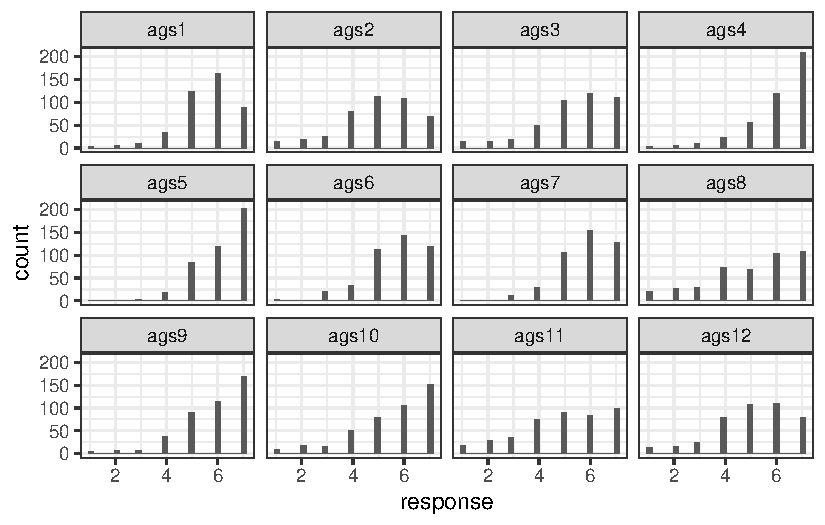
\includegraphics{./cfa_files/figure-pdf/unnamed-chunk-3-1.pdf}

}

\end{figure}

Seems like some questions have different means and variances from each
other. For example, the answers to \texttt{ags11} and \texttt{ags12} are
relatively flat, while the answers to \texttt{ags4} and \texttt{ags5}
are more bunched up around the highest values. The responses clearly
skew towards higher values in aggregate.

We can also do some healthy exploration of missingness in the dataset.
For starters: what proportion of values are missing in each row?

\begin{Shaded}
\begin{Highlighting}[]
\NormalTok{dat\_ags }\SpecialCharTok{\%\textgreater{}\%} 
  
  \CommentTok{\# Calculate the proportion of missing values }
  \FunctionTok{summarise\_all}\NormalTok{(}\SpecialCharTok{\textasciitilde{}} \FunctionTok{sum}\NormalTok{(}\FunctionTok{is.na}\NormalTok{(.)) }\SpecialCharTok{/}\NormalTok{ (}\FunctionTok{sum}\NormalTok{(}\FunctionTok{is.na}\NormalTok{(.) }\SpecialCharTok{+} \FunctionTok{sum}\NormalTok{(}\SpecialCharTok{!}\FunctionTok{is.na}\NormalTok{(.))))) }\SpecialCharTok{\%\textgreater{}\%} 
  
  \CommentTok{\# Rounding to make the results more presentable}
  \FunctionTok{mutate}\NormalTok{(}\FunctionTok{across}\NormalTok{(}\FunctionTok{everything}\NormalTok{(), round, }\DecValTok{6}\NormalTok{)) }\SpecialCharTok{\%\textgreater{}\%} 
  
  \CommentTok{\# Create the table}
\NormalTok{  knitr}\SpecialCharTok{::}\FunctionTok{kable}\NormalTok{(}\AttributeTok{title =} \StringTok{"Proportion of Missing Responses in Each Column"}\NormalTok{) }
\end{Highlighting}
\end{Shaded}

\begin{longtable}[]{@{}
  >{\raggedleft\arraybackslash}p{(\columnwidth - 22\tabcolsep) * \real{0.0870}}
  >{\raggedleft\arraybackslash}p{(\columnwidth - 22\tabcolsep) * \real{0.0652}}
  >{\raggedleft\arraybackslash}p{(\columnwidth - 22\tabcolsep) * \real{0.0652}}
  >{\raggedleft\arraybackslash}p{(\columnwidth - 22\tabcolsep) * \real{0.0870}}
  >{\raggedleft\arraybackslash}p{(\columnwidth - 22\tabcolsep) * \real{0.0870}}
  >{\raggedleft\arraybackslash}p{(\columnwidth - 22\tabcolsep) * \real{0.0870}}
  >{\raggedleft\arraybackslash}p{(\columnwidth - 22\tabcolsep) * \real{0.0870}}
  >{\raggedleft\arraybackslash}p{(\columnwidth - 22\tabcolsep) * \real{0.0870}}
  >{\raggedleft\arraybackslash}p{(\columnwidth - 22\tabcolsep) * \real{0.0870}}
  >{\raggedleft\arraybackslash}p{(\columnwidth - 22\tabcolsep) * \real{0.0870}}
  >{\raggedleft\arraybackslash}p{(\columnwidth - 22\tabcolsep) * \real{0.0870}}
  >{\raggedleft\arraybackslash}p{(\columnwidth - 22\tabcolsep) * \real{0.0870}}@{}}
\toprule()
\begin{minipage}[b]{\linewidth}\raggedleft
ags1
\end{minipage} & \begin{minipage}[b]{\linewidth}\raggedleft
ags2
\end{minipage} & \begin{minipage}[b]{\linewidth}\raggedleft
ags3
\end{minipage} & \begin{minipage}[b]{\linewidth}\raggedleft
ags4
\end{minipage} & \begin{minipage}[b]{\linewidth}\raggedleft
ags5
\end{minipage} & \begin{minipage}[b]{\linewidth}\raggedleft
ags6
\end{minipage} & \begin{minipage}[b]{\linewidth}\raggedleft
ags7
\end{minipage} & \begin{minipage}[b]{\linewidth}\raggedleft
ags8
\end{minipage} & \begin{minipage}[b]{\linewidth}\raggedleft
ags9
\end{minipage} & \begin{minipage}[b]{\linewidth}\raggedleft
ags10
\end{minipage} & \begin{minipage}[b]{\linewidth}\raggedleft
ags11
\end{minipage} & \begin{minipage}[b]{\linewidth}\raggedleft
ags12
\end{minipage} \\
\midrule()
\endhead
1.1e-05 & 5e-06 & 5e-06 & 1.6e-05 & 1.6e-05 & 1.1e-05 & 1.6e-05 &
1.6e-05 & 1.1e-05 & 2.2e-05 & 1.1e-05 & 1.6e-05 \\
\bottomrule()
\end{longtable}

That's very little missingness. Probably no need to do multiple
imputation here.

The authors also do a preliminary test of whether the responses are
normally distributed, since this is one of the fundamental assumptions
of maximum likelihood estimation. Kristoffer Magnusson has created
\href{https://rpsychologist.com/likelihood/}{a cool interactive teaching
tool that nicely illustrates this point}. It is worth remembering that
we \emph{do not} make this type of assumption for linear regression in
general -- only for maximum likelihood estimates. All we need assume for
linear regression is that the \emph{residuals} are normally distributed,
as opposed to the data themselves. This common misunderstanding can lead
researchers to commit what Richard McElreath has called
\href{https://stats.stackexchange.com/questions/515444/histomancy-what-does-mcelreath-propose-we-do-instead}{`histomancy'}.

To evaluate the assumption of normalness underlying maximum likelihood
estimation, the authors do what seems to be a multivariate version of a
classic `normal probability plot'. These are explained nicely in
\href{https://stats.stackexchange.com/questions/218638/understanding-normal-probability-plots}{this
stack exchange thread.} They also produce some of the classic tests of
skew and kurtosis, which I don't want to get into here.
\href{https://www.youtube.com/watch?v=TM033GCU-SY\&t=26s}{This youtuber}
has nice introductory videos about these topics.

\begin{Shaded}
\begin{Highlighting}[]
\CommentTok{\# Run the Mardia tests for normalness}
\NormalTok{mardia.object }\OtherTok{\textless{}{-}}\NormalTok{ psych}\SpecialCharTok{::}\FunctionTok{mardia}\NormalTok{(dat\_ags)}
\end{Highlighting}
\end{Shaded}

\begin{figure}[H]

{\centering 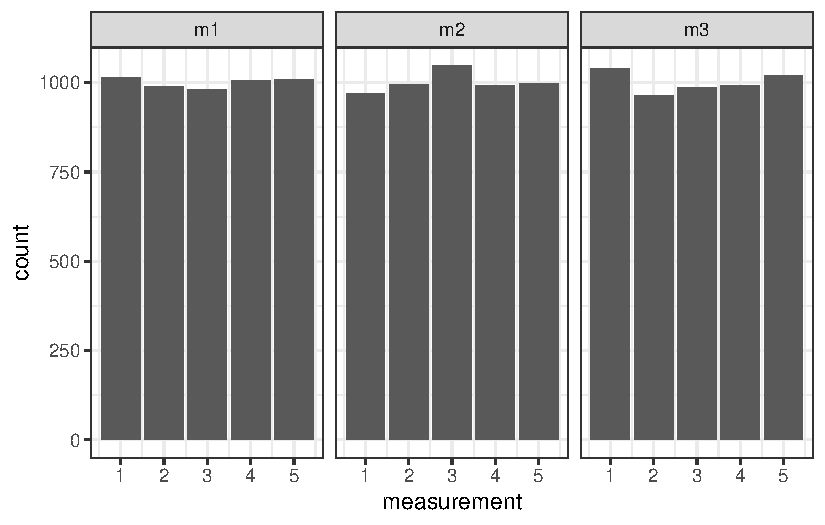
\includegraphics{./cfa_files/figure-pdf/unnamed-chunk-5-1.pdf}

}

\end{figure}

\begin{Shaded}
\begin{Highlighting}[]
\CommentTok{\# Plot the multivariate version of the normal probability plot}
\FunctionTok{plot}\NormalTok{(mardia.object)}

\CommentTok{\# Present the outputs we\textquotesingle{}re interested in}
\FunctionTok{tibble}\NormalTok{(}
  \StringTok{"Skew"} \OtherTok{=}\NormalTok{ mardia.object}\SpecialCharTok{$}\NormalTok{skew,}
  \StringTok{"Skew p{-}value"} \OtherTok{=}\NormalTok{ mardia.object}\SpecialCharTok{$}\NormalTok{p.skew,}
  \StringTok{"Kurtosis"} \OtherTok{=}\NormalTok{ mardia.object}\SpecialCharTok{$}\NormalTok{kurtosis,}
  \StringTok{"Kurtosis p{-}value"} \OtherTok{=}\NormalTok{ mardia.object}\SpecialCharTok{$}\NormalTok{p.kurt}
\NormalTok{) }\SpecialCharTok{\%\textgreater{}\%} 
  
\NormalTok{  knitr}\SpecialCharTok{::}\FunctionTok{kable}\NormalTok{()}
\end{Highlighting}
\end{Shaded}

\begin{longtable}[]{@{}rrrr@{}}
\toprule()
Skew & Skew p-value & Kurtosis & Kurtosis p-value \\
\midrule()
\endhead
2359.475 & 0 & 40.52999 & 0 \\
\bottomrule()
\end{longtable}

The plotted points don't seem to fit the straight line super well, which
suggests that the normalness assumption may not hold here. Also, the
hypothesis tests for skew and kurtosis return some mighty low p-values,
suggesting that we've got lots of each of them. So maybe maximum
likelihood estimation isn't such a good idea here?

The authors proceed with it anyway for pedogogical reasons, because they
want to illustrate how the maximum likelihood estimates differ from
estimates arrived at using other methods.

\begin{quote}
``In actual practice, given the lack of multivariate normality that
seems apparent in the previous results, we would likely not use ML and
instead rely on the alternative estimation approach.''
\end{quote}

\hypertarget{model-fitting}{%
\subsection{Model Fitting}\label{model-fitting}}

The researchers who collected the data do what good factor analysts do:
they look to the literature to set up some clear and specific candidate
hypotheses, and see the degree to which this new data is compatible with
each of them.

One of the candidate hypotheses is that a person's toxic striving energy
(`achievement goal orientedness'?) is secretly driven by four platonic
unobservable things, namely:

\begin{enumerate}
\def\labelenumi{\arabic{enumi}.}
\item
  Mastery Approach `MAP' (eg. \emph{``I want to learn as much as
  possible'')};
\item
  Mastery Avoidant `MAV' (eg. \emph{``I want to avoid learning less than
  I possibly could''});
\item
  Performance Approach `PAP' (eg. \emph{``I want to do well compared to
  other students'');}
\item
  Performance Avoidant `PAV' (eg. \emph{``It is important for me to
  avoid doing poorly compared to other students''})
\end{enumerate}

We'll call the above hypothesis \textbf{H1.} But there's another
hypothesis that says actually the `Mastery' variables are just one
monolithic thing, so really there are only 3 factors, namely `Mastery',
`PAP', and `PAV'. We'll call this one \textbf{H2.} These will be the two
candidate hypotheses we're gonna test via factor analysis.

The way \textbf{lavaan} works is that you need to separately define the
model syntax as a string, and then feed that string to one of the
model-fitting functions like \texttt{cfa()} . Then we can call the
\texttt{summary()} function to get a big table of outputs.

\begin{Shaded}
\begin{Highlighting}[]
\CommentTok{\# Define the relationships from my hypothesis}
\NormalTok{h1.definition }\OtherTok{\textless{}{-}} 
\StringTok{\textquotesingle{}map=\textasciitilde{}ags1+ags5+ags7}
\StringTok{mav=\textasciitilde{}ags2+ags6+ags12}
\StringTok{pap=\textasciitilde{}ags3+ags9+ags11}
\StringTok{pav=\textasciitilde{}ags4+ags8+ags10\textquotesingle{}}

\CommentTok{\# Fit the model}
\NormalTok{h1.fit }\OtherTok{\textless{}{-}} \FunctionTok{cfa}\NormalTok{(}
  \AttributeTok{data  =}\NormalTok{ dat\_ags,}
  \AttributeTok{model =}\NormalTok{ h1.definition}
\NormalTok{)}

\CommentTok{\# Look at the results}
\NormalTok{h1.summary }\OtherTok{\textless{}{-}} \FunctionTok{summary}\NormalTok{(h1.fit, }\AttributeTok{fit.measures =} \ConstantTok{TRUE}\NormalTok{, }\AttributeTok{standardized =} \ConstantTok{TRUE}\NormalTok{)}

\NormalTok{h1.summary}
\end{Highlighting}
\end{Shaded}

\begin{verbatim}
lavaan 0.6-12 ended normally after 48 iterations

  Estimator                                         ML
  Optimization method                           NLMINB
  Number of model parameters                        30

                                                  Used       Total
  Number of observations                           419         432

Model Test User Model:
                                                      
  Test statistic                               328.312
  Degrees of freedom                                48
  P-value (Chi-square)                           0.000

Model Test Baseline Model:

  Test statistic                              3382.805
  Degrees of freedom                                66
  P-value                                        0.000

User Model versus Baseline Model:

  Comparative Fit Index (CFI)                    0.915
  Tucker-Lewis Index (TLI)                       0.884

Loglikelihood and Information Criteria:

  Loglikelihood user model (H0)              -7014.070
  Loglikelihood unrestricted model (H1)      -6849.914
                                                      
  Akaike (AIC)                               14088.141
  Bayesian (BIC)                             14209.277
  Sample-size adjusted Bayesian (BIC)        14114.078

Root Mean Square Error of Approximation:

  RMSEA                                          0.118
  90 Percent confidence interval - lower         0.106
  90 Percent confidence interval - upper         0.130
  P-value RMSEA <= 0.05                          0.000

Standardized Root Mean Square Residual:

  SRMR                                           0.055

Parameter Estimates:

  Standard errors                             Standard
  Information                                 Expected
  Information saturated (h1) model          Structured

Latent Variables:
                   Estimate  Std.Err  z-value  P(>|z|)   Std.lv  Std.all
  map =~                                                                
    ags1              1.000                               0.840    0.746
    ags5              0.774    0.057   13.564    0.000    0.650    0.682
    ags7              1.100    0.064   17.263    0.000    0.924    0.895
  mav =~                                                                
    ags2              1.000                               0.923    0.627
    ags6              0.974    0.078   12.523    0.000    0.899    0.796
    ags12             1.039    0.096   10.805    0.000    0.959    0.644
  pap =~                                                                
    ags3              1.000                               1.284    0.840
    ags9              0.853    0.038   22.349    0.000    1.095    0.870
    ags11             1.103    0.052   21.178    0.000    1.416    0.841
  pav =~                                                                
    ags4              1.000                               0.929    0.771
    ags8              1.599    0.084   19.091    0.000    1.486    0.855
    ags10             1.525    0.073   20.861    0.000    1.418    0.921

Covariances:
                   Estimate  Std.Err  z-value  P(>|z|)   Std.lv  Std.all
  map ~~                                                                
    mav               0.709    0.079    9.000    0.000    0.914    0.914
    pap               0.066    0.060    1.093    0.274    0.061    0.061
    pav               0.056    0.043    1.289    0.197    0.072    0.072
  mav ~~                                                                
    pap               0.163    0.072    2.265    0.023    0.138    0.138
    pav               0.178    0.053    3.355    0.001    0.207    0.207
  pap ~~                                                                
    pav               1.143    0.102   11.236    0.000    0.958    0.958

Variances:
                   Estimate  Std.Err  z-value  P(>|z|)   Std.lv  Std.all
   .ags1              0.562    0.047   11.951    0.000    0.562    0.443
   .ags5              0.486    0.038   12.780    0.000    0.486    0.535
   .ags7              0.211    0.032    6.602    0.000    0.211    0.198
   .ags2              1.312    0.102   12.825    0.000    1.312    0.606
   .ags6              0.469    0.049    9.537    0.000    0.469    0.367
   .ags12             1.300    0.103   12.669    0.000    1.300    0.586
   .ags3              0.690    0.059   11.671    0.000    0.690    0.295
   .ags9              0.386    0.036   10.769    0.000    0.386    0.244
   .ags11             0.831    0.071   11.639    0.000    0.831    0.293
   .ags4              0.588    0.045   12.959    0.000    0.588    0.405
   .ags8              0.815    0.070   11.602    0.000    0.815    0.269
   .ags10             0.362    0.043    8.423    0.000    0.362    0.153
    map               0.706    0.083    8.514    0.000    1.000    1.000
    mav               0.852    0.128    6.655    0.000    1.000    1.000
    pap               1.648    0.158   10.416    0.000    1.000    1.000
    pav               0.864    0.094    9.198    0.000    1.000    1.000
\end{verbatim}

\begin{Shaded}
\begin{Highlighting}[]
\NormalTok{semPlot}\SpecialCharTok{::}\FunctionTok{semPaths}\NormalTok{(h1.fit)}
\end{Highlighting}
\end{Shaded}

\begin{figure}[H]

{\centering 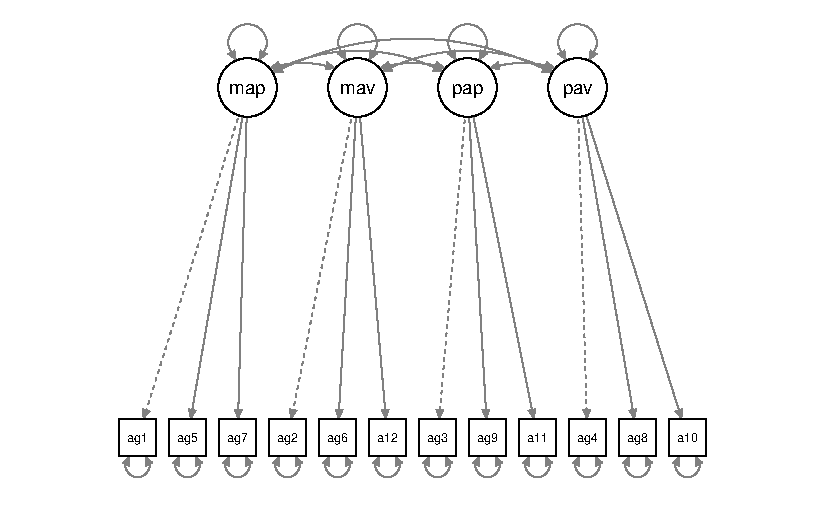
\includegraphics{./cfa_files/figure-pdf/unnamed-chunk-6-1.pdf}

}

\end{figure}

That's a lot of outputs. Let's break down the output into smaller
bite-sized chunks.

\hypertarget{goodness-of-fit-statistics}{%
\subsection{Goodness of Fit
Statistics}\label{goodness-of-fit-statistics}}

\hypertarget{chi-squared-statistic}{%
\subsubsection{Chi-Squared Statistic}\label{chi-squared-statistic}}

The first thing to look at is the chi-squared statistic from the `User
Model', IE the model I, the user, have just fit. I like to think of this
as a measure of how different the model's reconstructed correlation
matrix looks compared to the actual empirical correlation matrix of the
data. So we use this statistic to test the null hypothesis ``there is no
significant difference between model's reconstructed correlation matrix
and the empirical one''. So, confusingly, we're actually hoping to
\emph{accept} the null hypothesis here. This model returns a value of
328.312 with a vanishingly small p-value, so we reject the null
hypothesis, which is bad: it suggests our model isn't doing a good job
replicating the empirical correlation matrix.

Here's a quote from Gorsuch (1983) that explains this stuff from the
slightly different angle:

\begin{quote}
``The test of significance {[}for a CFA model fit by maximum
likelihood{]} gives a chi-square statistic with the null hypothesis
being that all the population covariance has been extracted by the
hypothesized number of factors. If the chi-square is significant at the
designated probability level, then the residual matrix still has
significant covariance in it.''
\end{quote}

So this chi-squared statistic provides a first look at goodness-of-fit,
but Finch (2015) say it is actually not very trustworthy in practice
because the null hypothesis is sort of crazy: we want a more permissive
test than just whether the model is \emph{perfectly} recreating the
empirical correlation matrix.

\begin{quote}
``this statistic is not particularly useful in practice because it tests
the null hypothesis that {[}the model-reconstructed correlation matrix
is equal to the empirical correlation matrix{]}, which is very
restrictive. The test will almost certainly be rejected when the sample
size is sufficiently large\ldots{} In addition, the chi-square test
relies on the assumption of multivariate normality of the indicators,
which may not be tenable in many situations.''
\end{quote}

So we're gonna wanna look at statistics other than just chi-squared for
goodness-of-fit, but it seems like a fine place to start. Let's look at
the chi-squared statistic of our model:

\begin{Shaded}
\begin{Highlighting}[]
\DocumentationTok{\#\#\# Create a nice summary table}
\FunctionTok{tibble}\NormalTok{(}
  \AttributeTok{Test             =} \StringTok{"standard chi{-}squared"}\NormalTok{,}
  \StringTok{\textasciigrave{}}\AttributeTok{DF}\StringTok{\textasciigrave{}}             \OtherTok{=}\NormalTok{ h1.summary}\SpecialCharTok{$}\NormalTok{test}\SpecialCharTok{$}\NormalTok{standard}\SpecialCharTok{$}\NormalTok{df,}
  \StringTok{\textasciigrave{}}\AttributeTok{Test Statistic}\StringTok{\textasciigrave{}} \OtherTok{=} \FunctionTok{round}\NormalTok{(h1.summary}\SpecialCharTok{$}\NormalTok{test}\SpecialCharTok{$}\NormalTok{standard}\SpecialCharTok{$}\NormalTok{stat, }\DecValTok{2}\NormalTok{),}
  \StringTok{\textasciigrave{}}\AttributeTok{p{-}value}\StringTok{\textasciigrave{}}        \OtherTok{=}\NormalTok{ h1.summary}\SpecialCharTok{$}\NormalTok{test}\SpecialCharTok{$}\NormalTok{standard}\SpecialCharTok{$}\NormalTok{pvalue}
\NormalTok{) }\SpecialCharTok{\%\textgreater{}\%} 
  
  \FunctionTok{mutate}\NormalTok{(}\FunctionTok{across}\NormalTok{(}\FunctionTok{everything}\NormalTok{(), as.character)) }\SpecialCharTok{\%\textgreater{}\%} 
  
  \FunctionTok{pivot\_longer}\NormalTok{(}\FunctionTok{everything}\NormalTok{()) }\SpecialCharTok{\%\textgreater{}\%} 
  
\NormalTok{  knitr}\SpecialCharTok{::}\FunctionTok{kable}\NormalTok{()}
\end{Highlighting}
\end{Shaded}

\begin{longtable}[]{@{}ll@{}}
\toprule()
name & value \\
\midrule()
\endhead
Test & standard chi-squared \\
DF & 48 \\
Test Statistic & 328.31 \\
p-value & 0 \\
\bottomrule()
\end{longtable}

It takes lots of skill and experience to have a sense of whether a test
statistic is big or small given the degrees of freedom at play, but we
can see from the p-value that we reject the null hypothesis in a big
way. This is bad -- it suggests that, given our assumptions, there's a
big difference between our model and the data.

\hypertarget{root-mean-squared-error-approximation-rmsea}{%
\subsubsection{Root Mean Squared Error Approximation
(RMSEA)}\label{root-mean-squared-error-approximation-rmsea}}

Another one people like to go with is the Root Mean Squared Error
Approximation (RMSEA). This statistic takes some math and background to
understand, which I'm not going to go over here. I found
\href{http://www.statpower.net/Content/312/Handout/Measures\%20of\%20Fit\%20in\%20Structural\%20Equation\%20Modeling.pdf}{this
document} to be the clearest (but also pretty mathy) explanation.

Essentially, RMSEA is a weighted sum of the discrepancies between the
model's reconstructed correlation matrix and the empirical correlation
matrix. But it also does a nice thing where it discounts model
complexity and sample size to help us not overfit. Here's the
definition:

\(\text{RMSEA} = \sqrt{\dfrac{χ^2 - \text{df}}{\text{df}(n-1)}}\)

See how it takes the chi-squared statistic and divides it by degrees of
freedom (as a proxy for model complexity) and sample size? This makes
for a more conservative measure of goodness-of-fit. Apparently the
square-root is used \emph{``to return the index to the same metric as
the original standardized parameters''}. I don't really understand that
part\ldots{} is it because a Chi-squared random variable is the squared
version of a normal standard variable?

As with the raw chi-squared statistic, we want RMSEA to be small because
it is intended as a measure of the distance between the empirical
correlation matrix and the model-estimated correlation matrix. According
to Finch (2015), people like to say:

\begin{itemize}
\item
  RMSEA \textless= 0.05 is a `good fit';
\item
  0.05 \textless{} RMSEA \textless= 0.08 is an `ok fit'
\item
  RMSEA \textgreater{} .08 is a `bad fit'.
\end{itemize}

Let's check the RMSEA of our model:

\begin{Shaded}
\begin{Highlighting}[]
\CommentTok{\# make a nice summary table}
\NormalTok{h1.summary}\SpecialCharTok{$}\NormalTok{fit }\SpecialCharTok{\%\textgreater{}\%} 
  
  \FunctionTok{as\_tibble}\NormalTok{(}\AttributeTok{rownames =} \StringTok{"stat"}\NormalTok{) }\SpecialCharTok{\%\textgreater{}\%} 
  
  \FunctionTok{filter}\NormalTok{(}\FunctionTok{str\_detect}\NormalTok{(stat, }\StringTok{"rmsea"}\NormalTok{)) }\SpecialCharTok{\%\textgreater{}\%} 
  
\NormalTok{  knitr}\SpecialCharTok{::}\FunctionTok{kable}\NormalTok{()}
\end{Highlighting}
\end{Shaded}

\begin{longtable}[]{@{}lr@{}}
\toprule()
stat & value \\
\midrule()
\endhead
rmsea & 0.1180574 \\
rmsea.ci.lower & 0.1061525 \\
rmsea.ci.upper & 0.1303058 \\
rmsea.pvalue & 0.0000000 \\
\bottomrule()
\end{longtable}

Yikes -- looks like our whole RMSEA, as well as its confidence interval,
are above the `bad fit' conventional threshold of .08. This corroborates
what we saw with the chi-squared statistic above.

\hypertarget{comparative-fit-index-cfi-and-tucker-lewis-index-tli}{%
\subsubsection{Comparative Fit Index (CFI) and Tucker-Lewis Index
(TLI)}\label{comparative-fit-index-cfi-and-tucker-lewis-index-tli}}

CFI seems to be the most trusted and widely-used tool for assessing
goodness of fit in a CFA. Basically the idea is that we ask: ``how much
does the chi-squared statistic of my model differ from the chi-squared
statistic of the worst model I can think of?'', where the conventional
``worst model I can think of'' is the model where I assume all of my
observed variables are totally uncorrelated. This sort of has the
opposite flavour of the deviance statistic I'm already familiar with,
which compares the current model with ``the best model I can think of.''

\(\text{CFI} = 1 - \dfrac{\text{max}(χ^2_T - \text{df}_T, 0)}{\text{max}(χ^2_0 - \text{df}_0, 0)}\)

Actually, the numerator and denominator are both equal to the
`non-centrality parameter' of their respective candidate distributions.
I'm not gonna get into this, but this is an idea that also shows up in
power analysis as a way of comparing the null and candidate hypotheses.

We want to end up with a CFI as close to 1 as possible, because that
suggests a big difference between my model and the worst possible model.
So people say we can sort of think of this as analogous to \(R^2\) from
linear regression. People seem to have adopted 0.95 as am arbitrary
cutoff for `good fit' for the CFI.

If you want to learn more about the CFI, I found
\href{https://scholarworks.umass.edu/cgi/viewcontent.cgi?article=1561\&context=pare}{this
article} a well-written resource.

Tucker-Lewis Index seems to be pretty similar to CFI, and we interpret
it in the same way. Let's look at both of them:

\begin{Shaded}
\begin{Highlighting}[]
\CommentTok{\# Make a nice summary table}
\NormalTok{h1.summary}\SpecialCharTok{$}\NormalTok{fit }\SpecialCharTok{\%\textgreater{}\%} 
  
  \FunctionTok{as\_tibble}\NormalTok{(}\AttributeTok{rownames =} \StringTok{"stat"}\NormalTok{) }\SpecialCharTok{\%\textgreater{}\%} 
  
  \FunctionTok{filter}\NormalTok{(}\FunctionTok{str\_detect}\NormalTok{(stat, }\StringTok{"cfi|tli"}\NormalTok{)) }\SpecialCharTok{\%\textgreater{}\%} 
  
\NormalTok{  knitr}\SpecialCharTok{::}\FunctionTok{kable}\NormalTok{()}
\end{Highlighting}
\end{Shaded}

\begin{longtable}[]{@{}lr@{}}
\toprule()
stat & value \\
\midrule()
\endhead
cfi & 0.9154874 \\
tli & 0.8837951 \\
\bottomrule()
\end{longtable}

Looks like the CFI and TLI look ok, but don't meet the conventional .95
cutoff. So they are in line with the chi-squared and RMSEA in suggesting
that our goodness-of-fit isn't so good.

\hypertarget{convergent-validty}{%
\subsection{Convergent Validty}\label{convergent-validty}}

When I'm doing factor analysis, my goal is to convince my research peers
that the observed variables are providing a way of measuring the
unobservable `factor' I'm purporting to exist. This seems like an
ontologically dubious framing, and it also seems impossible to prove.
But people who do research have settled on a few ways of trying to make
this case.

One such way is to take all of the measured variables I'm imagining to
be caused by the same unmeasured factor and show that they are indeed
correlated with each other. When this happens, I can say that my factor
has \textbf{Convergent Validity.} In the words of Gorsuch (1983):

\begin{quote}
\emph{``Convergent validity occurs when several variables deemed to
measure the same construct correlate with each other.''}
\end{quote}

Or, as Kline (2011) puts it:

\begin{quote}
\emph{``Variables presumed to measure the same construct show convergent
validity if their intercorrelations are appreciable in magnitude.''}
\end{quote}

So essentially I'm trying to make the case for a DAG where my observed
variables are all caused by a shared unobserved `latent' variable. It
seems like to make the jump from `these measured variables are
correlated' to `these measured variables are caused by a single shared
latent factor' I would need to be also making the further assumption
that there aren't \emph{other} unmeasured confounders muddying up the
observed covariances. It's DAGs all the way down\ldots{}

Based on the textbooks I'm working from, here are a few questions I can
answer if I want to make the case for Convergent Validity:

\begin{enumerate}
\def\labelenumi{\arabic{enumi}.}
\tightlist
\item
  Are the factor loadings statistically significant?
\item
  Are the standardized factor loadings pretty big (IE pretty close to
  1)?
\item
  Are the within-factor loadings pretty similar to each other?
\item
  Do the measurements seem to have good `reliability' as measured by
  something like Chronbach's Alpha, Average Variance Extracted, or
  Composite Reliability?
\item
  Are all of the residual variances less than .50, IE is the model
  explaining at least half the variance of each model?
\end{enumerate}

First we can look at the factor loadings. These are essentially just the
regression coefficients of each factor on each of the outcome variables
for which it was allowed to be a covariate. So we want them to be big
and significant.

\begin{Shaded}
\begin{Highlighting}[]
\DocumentationTok{\#\#\# Make a nice summary table of the factor loadings}
\NormalTok{h1.summary}\SpecialCharTok{$}\NormalTok{pe }\SpecialCharTok{\%\textgreater{}\%} 
  
  \FunctionTok{as\_tibble}\NormalTok{() }\SpecialCharTok{\%\textgreater{}\%} 
  
  \CommentTok{\# Keep only the rows with info on factor loadings}
  \FunctionTok{slice}\NormalTok{(}\DecValTok{1}\SpecialCharTok{:}\DecValTok{12}\NormalTok{) }\SpecialCharTok{\%\textgreater{}\%} 
  
  \CommentTok{\# Clean up the important values, then combine them into a single column}
  \FunctionTok{mutate}\NormalTok{(}
    \AttributeTok{std.all =} \FunctionTok{round}\NormalTok{(std.all, }\DecValTok{2}\NormalTok{),}
    \AttributeTok{std.all =} \FunctionTok{paste0}\NormalTok{(std.all, }\StringTok{", pvalue = "}\NormalTok{, pvalue, }\StringTok{")"}\NormalTok{)}
\NormalTok{  ) }\SpecialCharTok{\%\textgreater{}\%} 
  
  \CommentTok{\# reformat the table}
  \FunctionTok{select}\NormalTok{(lhs, rhs, std.all) }\SpecialCharTok{\%\textgreater{}\%} 
  
  \FunctionTok{pivot\_wider}\NormalTok{(}
    \AttributeTok{names\_from =} \StringTok{"lhs"}\NormalTok{, }
    \AttributeTok{values\_from =} \StringTok{"std.all"}\NormalTok{,}
    \AttributeTok{values\_fill =} \StringTok{"0"}
\NormalTok{  ) }\SpecialCharTok{\%\textgreater{}\%} 
  
  \FunctionTok{column\_to\_rownames}\NormalTok{(}\StringTok{"rhs"}\NormalTok{) }\SpecialCharTok{\%\textgreater{}\%} 
  
\NormalTok{  knitr}\SpecialCharTok{::}\FunctionTok{kable}\NormalTok{(}\AttributeTok{caption =} \StringTok{"Standardized factor loadings and p{-}values"}\NormalTok{)}
\end{Highlighting}
\end{Shaded}

\begin{longtable}[]{@{}
  >{\raggedright\arraybackslash}p{(\columnwidth - 8\tabcolsep) * \real{0.0732}}
  >{\raggedright\arraybackslash}p{(\columnwidth - 8\tabcolsep) * \real{0.2317}}
  >{\raggedright\arraybackslash}p{(\columnwidth - 8\tabcolsep) * \real{0.2317}}
  >{\raggedright\arraybackslash}p{(\columnwidth - 8\tabcolsep) * \real{0.2317}}
  >{\raggedright\arraybackslash}p{(\columnwidth - 8\tabcolsep) * \real{0.2317}}@{}}
\caption{Standardized factor loadings and p-values}\tabularnewline
\toprule()
\begin{minipage}[b]{\linewidth}\raggedright
\end{minipage} & \begin{minipage}[b]{\linewidth}\raggedright
map
\end{minipage} & \begin{minipage}[b]{\linewidth}\raggedright
mav
\end{minipage} & \begin{minipage}[b]{\linewidth}\raggedright
pap
\end{minipage} & \begin{minipage}[b]{\linewidth}\raggedright
pav
\end{minipage} \\
\midrule()
\endfirsthead
\toprule()
\begin{minipage}[b]{\linewidth}\raggedright
\end{minipage} & \begin{minipage}[b]{\linewidth}\raggedright
map
\end{minipage} & \begin{minipage}[b]{\linewidth}\raggedright
mav
\end{minipage} & \begin{minipage}[b]{\linewidth}\raggedright
pap
\end{minipage} & \begin{minipage}[b]{\linewidth}\raggedright
pav
\end{minipage} \\
\midrule()
\endhead
ags1 & 0.75, pvalue = NA) & 0 & 0 & 0 \\
ags5 & 0.68, pvalue = 0) & 0 & 0 & 0 \\
ags7 & 0.9, pvalue = 0) & 0 & 0 & 0 \\
ags2 & 0 & 0.63, pvalue = NA) & 0 & 0 \\
ags6 & 0 & 0.8, pvalue = 0) & 0 & 0 \\
ags12 & 0 & 0.64, pvalue = 0) & 0 & 0 \\
ags3 & 0 & 0 & 0.84, pvalue = NA) & 0 \\
ags9 & 0 & 0 & 0.87, pvalue = 0) & 0 \\
ags11 & 0 & 0 & 0.84, pvalue = 0) & 0 \\
ags4 & 0 & 0 & 0 & 0.77, pvalue = NA) \\
ags8 & 0 & 0 & 0 & 0.85, pvalue = 0) \\
ags10 & 0 & 0 & 0 & 0.92, pvalue = 0) \\
\bottomrule()
\end{longtable}

Firstly, notice that all of the non-fixed loadings are highly
statistically significant, with all p-values smaller than .01. This is
good! Super statistically-significant loadings are a necessary sign that
our measured variables are actually good proxies for the imaginary
`latent' factor we're purporting to use them to measure.

Next, Kline (2011) says that we can start assessing convergent validity
by just looking at the standardized loadings can in isolation. In his
words on page 344:

\begin{quote}
\emph{``{[}with reference to a CFA model he has fit{]}: A few other
standardized coefficients are rather low, such as .433 for the self-talk
indicator of constructive thinking, so evidence for convergent validity
is mixed.''}
\end{quote}

To my eye it looks like some of the standardized loadings on the `mav'
factor are pretty low. Also, it seems like only `pap' has really
consistent loadings across all of its measured variables: the other
three factors all have a bunch of variance between their loadings. So
this all seems like a bit of a red flag.

Next we can look at measures of \textbf{reliability,} which neither
Gorsuch (1983) nor Finch (2015) mention. This is a concept based on the
assumption from classical test theory that every datapoint is the sum of
a `true' score and `noise', where the `true' score is the value of the
latent variable. This is an ontologically dubious framing, but I guess a
useful or at least traditional one. Anyway, people like to do things in
hopes of estimating the proportion of the variance explained by the
`true' score as opposed to noise, and when they do these things they say
they are estimating `reliability'. Ok.

The all-time classic `reliability' measure is called \textbf{Cronbach's
Alpha.} Cronbach didn't actually invent it, so hello
\href{https://en.wikipedia.org/wiki/Stigler\%27s_law_of_eponymy}{Stigler's
Law}. Here's what it looks like:

\(\alpha = (\dfrac{k}{1-k}) (1 - \dfrac{\sum\sigma_y^2}{\sigma_T^2})\)

The term on the right is doing most of the work: its denominator is the
variance of the column that contains the rowwise sums of my dataset. Its
numerator is the sum of the variances of each column. So we're asking:
`is the variance of the \emph{sums} larger than the variance of the
individual columns?' This will be true if the columns are generally
pretty correlated, because the sums will \emph{stack up} the raw values,
instead of them cancelling each other out. So really we're just asking:
are the columns generally pretty correlated?`. If my columns are pretty
correlated and I make the standard assumption that \emph{no other latent
factors are influencing my observed values} (an insane assumption), then
I can feel comfortable saying that Cronbach's Alpha is useful for
figuring out whether my measurements are all loading on the same
'latent' variable. Since the observed values are gonna be consistent
with each other if this is true, people like to say that Cronbach's
Alpha gives a picture of \textbf{`Internal Consistency Reliability'.}

As with everything related to convergent validity, this is just another
way of asking how correlated my measured variables are.

Let's calculate Cronbach's Alpha for each of the subscales I've used to
define my supposed factors:

\begin{Shaded}
\begin{Highlighting}[]
\DocumentationTok{\#\#\# Split the dataset into the subscales assumed by my factor model}
\NormalTok{subscales }\OtherTok{\textless{}{-}} \FunctionTok{list}\NormalTok{(}
  \AttributeTok{map =}\NormalTok{ dat\_ags }\SpecialCharTok{\%\textgreater{}\%} \FunctionTok{select}\NormalTok{(ags1, ags5, ags7),}
  \AttributeTok{mav =}\NormalTok{ dat\_ags }\SpecialCharTok{\%\textgreater{}\%} \FunctionTok{select}\NormalTok{(ags2, ags6, ags12),}
  \AttributeTok{pap =}\NormalTok{ dat\_ags }\SpecialCharTok{\%\textgreater{}\%} \FunctionTok{select}\NormalTok{(ags3, ags9, ags11),}
  \AttributeTok{pav =}\NormalTok{ dat\_ags }\SpecialCharTok{\%\textgreater{}\%} \FunctionTok{select}\NormalTok{(ags4, ags8, ags10)}
\NormalTok{)}

\DocumentationTok{\#\#\# Calculate Chronbach\textquotesingle{}s Alpha for each subscale, then analyze.}
\NormalTok{alphas }\OtherTok{\textless{}{-}}\NormalTok{ subscales }\SpecialCharTok{\%\textgreater{}\%} 
  
  \FunctionTok{map}\NormalTok{(psych}\SpecialCharTok{::}\NormalTok{alpha) }\SpecialCharTok{\%\textgreater{}\%} 
  
  \FunctionTok{map}\NormalTok{(summary) }\SpecialCharTok{\%\textgreater{}\%} 
  
\NormalTok{  knitr}\SpecialCharTok{::}\FunctionTok{kable}\NormalTok{() }
\end{Highlighting}
\end{Shaded}

\begin{verbatim}

Reliability analysis   
 raw_alpha std.alpha G6(smc) average_r S/N   ase mean  sd median_r
      0.82      0.82    0.76       0.6 4.6 0.015  5.9 0.9      0.6

Reliability analysis   
 raw_alpha std.alpha G6(smc) average_r S/N   ase mean  sd median_r
      0.77      0.77    0.71      0.52 3.3 0.018  5.3 1.2     0.45

Reliability analysis   
 raw_alpha std.alpha G6(smc) average_r S/N    ase mean  sd median_r
      0.88      0.89    0.84      0.73 7.9 0.0095  5.4 1.3     0.74

Reliability analysis   
 raw_alpha std.alpha G6(smc) average_r S/N  ase mean  sd median_r
      0.87      0.88    0.85       0.7 7.1 0.01  5.6 1.3     0.72
\end{verbatim}

According to Kline (2011), these all look like good results, so they
help me feel good about claiming convergent validity:

\begin{quote}
``Generally, coefficients around .90 are considered''excellent,'' values
around .80 as ``very good,'' and values about .70 as ``adequate.''''
\end{quote}

Cronbach's Alpha has some drawbacks as a measure of `reliability', so
Kline (2011) says to also calculate the \textbf{Average Variance
Extracted (AVE)}, which is simply the average of the within-factor
squared factor loadings. This is based on the idea that a squared factor
loading is the variance explained of the variable by that factor. The
convention is that if the AVE \textgreater{} 0.5, then you can feel good
about claiming convergent validity. I guess this makes sense -- seems
like a pretty simple and ad-hoc way of asking whether your loadings are
generally on the same page. But obviously if I have lots of observed
variables defining the factor then I'm at risk of having a bunch of high
loadings and a bunch of low loadings, resulting in a misleadingly
moderate average? To me it seems like we might as well just look at the
raw loadings themselves -- no need to look at an average here.

But just for fun, let's calculate the AVE. Rather than doing it
manually, we can use a ready-made function from the \textbf{semTools}
package

\begin{Shaded}
\begin{Highlighting}[]
\NormalTok{semTools}\SpecialCharTok{::}\FunctionTok{AVE}\NormalTok{(h1.fit) }\SpecialCharTok{\%\textgreater{}\%} 
  
\NormalTok{  knitr}\SpecialCharTok{::}\FunctionTok{kable}\NormalTok{()}
\end{Highlighting}
\end{Shaded}

\begin{longtable}[]{@{}lr@{}}
\toprule()
& x \\
\midrule()
\endhead
map & 0.6115914 \\
mav & 0.4556936 \\
pap & 0.7179750 \\
pav & 0.7422385 \\
\bottomrule()
\end{longtable}

Based on the rule-of-thumb that we want the AVE to be at least .50, it
seems like the `mav' factor is having some trouble. It also had the
lowest Cronbach Alpha. So maybe the observed variables I'm using to
measure it aren't actually doing a great job? This hurts convergent
validity for that factor.

Lastly, we can also try to measure this unicorn of `reliability' by just
directly asking ``what proportion of the total variance is explained by
the factor model?''. People like to do this by summing all the factor
loadings, squaring that sum, and dividing it by itself plus the sum of
the residual variances of the variables (IE dividing it by the total
empirical variance of the variable). They call this one the
\textbf{Composite Reliability (CR).}

\begin{Shaded}
\begin{Highlighting}[]
\NormalTok{semTools}\SpecialCharTok{::}\FunctionTok{compRelSEM}\NormalTok{(h1.fit) }\SpecialCharTok{\%\textgreater{}\%} 
  
\NormalTok{  knitr}\SpecialCharTok{::}\FunctionTok{kable}\NormalTok{()}
\end{Highlighting}
\end{Shaded}

\begin{longtable}[]{@{}lr@{}}
\toprule()
& x \\
\midrule()
\endhead
map & 0.8164263 \\
mav & 0.6689921 \\
pap & 0.8803380 \\
pav & 0.9016062 \\
\bottomrule()
\end{longtable}

Apparently the rule of thumb for this one is the same as for Cronbach's
Alpha. So we can feel good about all of them except for `mav', which has
taken a beating via these 3 checks.

Kline (2011), on page 307, gives yet another way of assessing convergent
validity: he fits a CFA, then asks whether ``the majority'' of the
variances of the observed variables have been explained, IE whether the
standardized residual variances are \textless50. I guess the idea is
that the amount of variance explained for a variable by a factor depends
on how correlated In his words:

\begin{quote}
``{[}in reference to one of his models:{]} {[}the{]} model fails to
explain the majority (\textgreater{} .50) of variance for a total of
four out of eight indicators, which indicates poor convergent
validity.''
\end{quote}

Let's have a look at the residual variances. These are just the
proportion of the empirical variance of each measured variable that is
left unexplained by the linear models that make up the factor analysis.

\begin{Shaded}
\begin{Highlighting}[]
\NormalTok{h1.summary}\SpecialCharTok{$}\NormalTok{pe }\SpecialCharTok{\%\textgreater{}\%} 
  
  \FunctionTok{as.data.frame}\NormalTok{() }\SpecialCharTok{\%\textgreater{}\%} 
  
  \FunctionTok{filter}\NormalTok{(}\FunctionTok{grepl}\NormalTok{(}\StringTok{"ags}\SpecialCharTok{\textbackslash{}\textbackslash{}}\StringTok{d"}\NormalTok{, lhs)) }\SpecialCharTok{\%\textgreater{}\%} 
  
  \FunctionTok{mutate}\NormalTok{(}\AttributeTok{factor =} \FunctionTok{case\_when}\NormalTok{(}
\NormalTok{    lhs }\SpecialCharTok{\%in\%} \FunctionTok{c}\NormalTok{(}\StringTok{"ags1"}\NormalTok{, }\StringTok{"ags5"}\NormalTok{, }\StringTok{"ags7"}\NormalTok{) }\SpecialCharTok{\textasciitilde{}} \StringTok{"map"}\NormalTok{,}
\NormalTok{    lhs }\SpecialCharTok{\%in\%} \FunctionTok{c}\NormalTok{(}\StringTok{"ags2"}\NormalTok{, }\StringTok{"ags6"}\NormalTok{, }\StringTok{"ags12"}\NormalTok{) }\SpecialCharTok{\textasciitilde{}} \StringTok{"mav"}\NormalTok{,}
\NormalTok{    lhs }\SpecialCharTok{\%in\%} \FunctionTok{c}\NormalTok{(}\StringTok{"ags3"}\NormalTok{, }\StringTok{"ags9"}\NormalTok{, }\StringTok{"ags11"}\NormalTok{) }\SpecialCharTok{\textasciitilde{}} \StringTok{"pap"}\NormalTok{,}
\NormalTok{    lhs }\SpecialCharTok{\%in\%} \FunctionTok{c}\NormalTok{(}\StringTok{"ags4"}\NormalTok{, }\StringTok{"ags8"}\NormalTok{, }\StringTok{"ags10"}\NormalTok{) }\SpecialCharTok{\textasciitilde{}} \StringTok{"pav"}\NormalTok{,}
\NormalTok{  )) }\SpecialCharTok{\%\textgreater{}\%} 
  
  \FunctionTok{select}\NormalTok{(factor, }\StringTok{"var"} \OtherTok{=}\NormalTok{ lhs, std.all) }\SpecialCharTok{\%\textgreater{}\%} 
  
\NormalTok{  knitr}\SpecialCharTok{::}\FunctionTok{kable}\NormalTok{()}
\end{Highlighting}
\end{Shaded}

\begin{longtable}[]{@{}llr@{}}
\toprule()
factor & var & std.all \\
\midrule()
\endhead
map & ags1 & 0.4434896 \\
map & ags5 & 0.5345470 \\
map & ags7 & 0.1980907 \\
mav & ags2 & 0.6063553 \\
mav & ags6 & 0.3670913 \\
mav & ags12 & 0.5858185 \\
pap & ags3 & 0.2950189 \\
pap & ags9 & 0.2436200 \\
pap & ags11 & 0.2927905 \\
pav & ags4 & 0.4050030 \\
pav & ags8 & 0.2694999 \\
pav & ags10 & 0.1526773 \\
\bottomrule()
\end{longtable}

Looks like the model has mostly done a good job for the `Performance'
factors, with all variables having at least \textasciitilde60\% of their
variance explained. But the `Mastery' factors are worse, especially
`mav', with two of its three variables having only \textasciitilde40\%
of their variances explained. This is yet more evidence that the `mav'
factor isn't doing so great a job.

\textasciitilde\textasciitilde Lastly, Gorsuch suggests another way of
testing for convergent validity:

\begin{quote}
\emph{factor loadings of several variables hypothesized to relate to the
construct can also be tested for significance. They could be specified
as equal for the one model and the chi-square for that model subtracted
from another hypothesized factor structure where they are allowed to
vary. If the two differ significantly from each other, then one or more
of the variables is more related to the construct than one or more of
the other variables.''}
\end{quote}

Let's try this out: we'll fit another model that assumes all of the
within-factor loadings are equal, and see if that results in a
statistically significant reduction in goodness-of-fit. If it does, then
we lose some evidence of convergent
validity.\textasciitilde\textasciitilde{}

\hypertarget{discriminant-validity}{%
\subsection{Discriminant Validity}\label{discriminant-validity}}

Next let's look at the estimated correlations between the factors. If my
hypothesis H1 is true then we should expect all of the factors to be
pretty uncorrelated from each other, but if H2 is true then we should
expect MAP and MAV to be super correlated with each other, because H2
thinks there's no such thing as MAP and MAV -- there's just one big
`Mastery' factor:

\begin{Shaded}
\begin{Highlighting}[]
\DocumentationTok{\#\#\# Make a nicer version of the correlation matrix of the factors}
  
\NormalTok{h1.summary}\SpecialCharTok{$}\NormalTok{pe }\SpecialCharTok{\%\textgreater{}\%} 
  
  \FunctionTok{as\_tibble}\NormalTok{() }\SpecialCharTok{\%\textgreater{}\%} 
 
  \CommentTok{\# Keep only the rows with info on factor loadings}
  \FunctionTok{slice}\NormalTok{(}\DecValTok{25}\SpecialCharTok{:}\DecValTok{34}\NormalTok{) }\SpecialCharTok{\%\textgreater{}\%} 
 
  \FunctionTok{select}\NormalTok{(lhs, rhs, std.lv) }\SpecialCharTok{\%\textgreater{}\%} 
  
  \FunctionTok{mutate}\NormalTok{(}
    \AttributeTok{std.lv =} \FunctionTok{round}\NormalTok{(std.lv, }\DecValTok{2}\NormalTok{),}
    \FunctionTok{across}\NormalTok{(}\FunctionTok{everything}\NormalTok{(), as.character)}
\NormalTok{  ) }\SpecialCharTok{\%\textgreater{}\%} 
  
  \FunctionTok{pivot\_wider}\NormalTok{(}
    \AttributeTok{names\_from =} \StringTok{"lhs"}\NormalTok{, }
    \AttributeTok{values\_from =} \StringTok{"std.lv"}\NormalTok{,}
    \AttributeTok{values\_fill =} \StringTok{" "} 
\NormalTok{  ) }\SpecialCharTok{\%\textgreater{}\%} 
  
  \FunctionTok{column\_to\_rownames}\NormalTok{(}\StringTok{"rhs"}\NormalTok{) }\SpecialCharTok{\%\textgreater{}\%} 
  
\NormalTok{  knitr}\SpecialCharTok{::}\FunctionTok{kable}\NormalTok{(}\AttributeTok{caption =} \StringTok{"Correlation matrix of the factors"}\NormalTok{)}
\end{Highlighting}
\end{Shaded}

\begin{longtable}[]{@{}lllll@{}}
\caption{Correlation matrix of the factors}\tabularnewline
\toprule()
& map & mav & pap & pav \\
\midrule()
\endfirsthead
\toprule()
& map & mav & pap & pav \\
\midrule()
\endhead
map & 1 & & & \\
mav & 0.91 & 1 & & \\
pap & 0.06 & 0.14 & 1 & \\
pav & 0.07 & 0.21 & 0.96 & 1 \\
\bottomrule()
\end{longtable}

Interesting -- the `Mastery' factors and the `Performance' factors each
seem to be very correlated with each other, while being nice and
uncorrelated with the two factors that make up the other. This suggests
that we have bad \textbf{discriminant validity} between the imagined two
types of `Mastery' and two types of `Performance' -- the model can't
really tell them apart as separate things. This makes it harder for me
to argue that they \emph{are} in fact separate things. But then again,
maybe my hypothesis is that the within-skill factors \emph{should} be
highly correlated. Anyhow, the fact that the `Mastery' and `Performance'
factors are all pretty uncorrelated with each other is a good thing for
both hypotheses.

Brown (2006) gives some nice advice about how to assess discriminant
validty, and how to deal with it if you have it:

\begin{quote}
``In applied research, a factor correlation that exceeds .80 or .85 is
often used as the criterion to define poor discriminant validity. When
two factors are highly overlapping, a common research strategy is to
respecify the model by collapsing the dimensions into a single factor
and determine whether this modification results in a significant
degradation in model fit. If the respecified model provides an
acceptable fit to the data, it is usually favored because of its
superior parsimony.''

Gorsuch (1983) suggests doing something similar:
\end{quote}

\begin{quote}
\emph{``{[}fit the model{]} with the qualification that the correlations
between one or more of the constructs being tested for discriminant
validity is one. The difference between chi-squares from {[}this model
vs the model where the correlations are allowed to freely vary{]} tests
whether the constructs have a correlation significantly less than 1.0.
If the correlation between the factors for the two constructs is not
significantly different from 1.0, the difference chi-square will be
insignificant. This means the null hypothesis of no discriminatory
validity would be accepted. If the difference chi-square is significant,
then the null hypothesis is rejected and the model that assumes
discriminatory validity by allowing the correlation to be less than one
is the more appropriate one.''}
\end{quote}

This has the flavour of a likelihood-ratio test. Let's do it. First we
need to fit the model where the correlation between the Mastery factors
and the correlation between the `Performance' factors are both
constrained to be 1:

\begin{Shaded}
\begin{Highlighting}[]
\CommentTok{\# Define the relationships from my hypothesis}
\NormalTok{h1\_orthogonal.definition }\OtherTok{\textless{}{-}} 
\StringTok{\textquotesingle{}map=\textasciitilde{}ags1+ags5+ags7}
\StringTok{mav=\textasciitilde{}ags2+ags6+ags12}
\StringTok{pap=\textasciitilde{}ags3+ags9+ags11}
\StringTok{pav=\textasciitilde{}ags4+ags8+ags10}

\StringTok{map \textasciitilde{}\textasciitilde{} 1*mav}
\StringTok{pap \textasciitilde{}\textasciitilde{} 1*pav}
\StringTok{\textquotesingle{}}

\CommentTok{\# Fit the model}
\NormalTok{h1\_orthogonal.fit }\OtherTok{\textless{}{-}} \FunctionTok{cfa}\NormalTok{(}
  \AttributeTok{data  =}\NormalTok{ dat\_ags,}
  \AttributeTok{model =}\NormalTok{ h1\_orthogonal.definition}
\NormalTok{)}

\CommentTok{\# Compare the goodness{-}of{-}fit statistics for the two models}
\FunctionTok{anova}\NormalTok{(h1.fit, h1\_orthogonal.fit) }\SpecialCharTok{\%\textgreater{}\%} 
  
\NormalTok{  knitr}\SpecialCharTok{::}\FunctionTok{kable}\NormalTok{()}
\end{Highlighting}
\end{Shaded}

\begin{longtable}[]{@{}
  >{\raggedright\arraybackslash}p{(\columnwidth - 14\tabcolsep) * \real{0.2308}}
  >{\raggedleft\arraybackslash}p{(\columnwidth - 14\tabcolsep) * \real{0.0385}}
  >{\raggedleft\arraybackslash}p{(\columnwidth - 14\tabcolsep) * \real{0.1154}}
  >{\raggedleft\arraybackslash}p{(\columnwidth - 14\tabcolsep) * \real{0.1154}}
  >{\raggedleft\arraybackslash}p{(\columnwidth - 14\tabcolsep) * \real{0.1154}}
  >{\raggedleft\arraybackslash}p{(\columnwidth - 14\tabcolsep) * \real{0.1410}}
  >{\raggedleft\arraybackslash}p{(\columnwidth - 14\tabcolsep) * \real{0.1026}}
  >{\raggedleft\arraybackslash}p{(\columnwidth - 14\tabcolsep) * \real{0.1410}}@{}}
\toprule()
\begin{minipage}[b]{\linewidth}\raggedright
\end{minipage} & \begin{minipage}[b]{\linewidth}\raggedleft
Df
\end{minipage} & \begin{minipage}[b]{\linewidth}\raggedleft
AIC
\end{minipage} & \begin{minipage}[b]{\linewidth}\raggedleft
BIC
\end{minipage} & \begin{minipage}[b]{\linewidth}\raggedleft
Chisq
\end{minipage} & \begin{minipage}[b]{\linewidth}\raggedleft
Chisq diff
\end{minipage} & \begin{minipage}[b]{\linewidth}\raggedleft
Df diff
\end{minipage} & \begin{minipage}[b]{\linewidth}\raggedleft
Pr(\textgreater Chisq)
\end{minipage} \\
\midrule()
\endhead
h1.fit & 48 & 14088.14 & 14209.28 & 328.3120 & NA & NA & NA \\
h1\_orthogonal.fit & 50 & 14096.44 & 14209.50 & 340.6065 & 12.29456 & 2
& 0.0021393 \\
\bottomrule()
\end{longtable}

Looks like the reduction in chi-squared goodness-of-fit is statistically
significant when we force the within-skill factors to be perfectly
correlated. So, according to the Gorsuch (1983) quote above, we can
reject the null hypothesis that the within-skill factors are perfectly
correlated. This gives a justification for continuing to distinguish
between them as separate factors, and helps me make a believable claim
that my posited factors are in fact different things.

Actually, I think another way we could have done this would be to just
fit the model where we just define one big factor for `Mastery' and one
big factor for `Performance'. I tried this and it returned even worse
fit, which means the extra parameters (the correlation parameters) are
significantly improving fit in the pure h1 model.

\hypertarget{conclusion}{%
\subsection{Conclusion}\label{conclusion}}

All-in-all it seems like neither of these hypotheses do a great job.
Sure, the `Performance' factors have good convergent validity, and we
see good discriminant validity between the `Performance' and `Mastery'
factors, but the `Mastery' factors don't have great convergent validity
and fitting a single monolithic `Mastery' factor doesn't improve things.

I can make a better model by dropping the measured `Mastery' variables
that aren't having lots of their variance explained by the `Mastery'
factors, but this is contrary to the spirit of CFA. If I want to test a
different hypothesis then I should collect a different sample.

For a nice template of a more formal presentation of the results of a
CFA, see Brown (2006) chapter 4 appendix 3.

\hypertarget{example-2-biodiversity}{%
\section{Example 2: Biodiversity}\label{example-2-biodiversity}}

Here's
\href{https://d9-wret.s3.us-west-2.amazonaws.com/assets/palladium/production/s3fs-public/atoms/files/SEM_09_2-Ex1_CFA_exercise.pdf}{a
fun example from the Wetland and Aquatic Research Center of the U.S.
Geological Survey}: given counts of different types of animals, can we
fit a convincing CFA model for `diversity'? In other words: is the
correlation structure of all my counts of various types of animals
consistent with the possibility that those counts are confounded by a
single unobserved thing called `diversity'?

\begin{Shaded}
\begin{Highlighting}[]
\NormalTok{dat\_raw }\OtherTok{\textless{}{-}} \FunctionTok{read.csv}\NormalTok{(}\StringTok{\textquotesingle{}data/grace/SEM\_09\_2{-}Ex1\_CFA\_exercise\_data.csv\textquotesingle{}}\NormalTok{)}

\NormalTok{dat\_clean }\OtherTok{\textless{}{-}}\NormalTok{ dat\_raw }\SpecialCharTok{\%\textgreater{}\%}  
  
\NormalTok{  janitor}\SpecialCharTok{::}\FunctionTok{clean\_names}\NormalTok{()}
\end{Highlighting}
\end{Shaded}

\hypertarget{data-exploration-1}{%
\subsection{Data Exploration}\label{data-exploration-1}}

Just for fun let's see if the relative proportions of the different
animals varies between countries:

\begin{Shaded}
\begin{Highlighting}[]
\DocumentationTok{\#\#\# Proportions}
\NormalTok{dat\_clean }\SpecialCharTok{\%\textgreater{}\%} 
  
  \FunctionTok{pivot\_longer}\NormalTok{(}
    \AttributeTok{cols      =} \SpecialCharTok{!}\FunctionTok{matches}\NormalTok{(}\StringTok{"\^{}c"}\NormalTok{),}
    \AttributeTok{names\_to  =} \StringTok{"animal"}\NormalTok{,}
    \AttributeTok{values\_to =} \StringTok{"count"}
\NormalTok{  ) }\SpecialCharTok{\%\textgreater{}\%} 
  
  \FunctionTok{group\_by}\NormalTok{(country) }\SpecialCharTok{\%\textgreater{}\%} 
  \FunctionTok{mutate}\NormalTok{(}
    \AttributeTok{total =} \FunctionTok{sum}\NormalTok{(count), }
    \AttributeTok{prop  =} \FunctionTok{round}\NormalTok{(count }\SpecialCharTok{/}\NormalTok{ total, }\DecValTok{2}\NormalTok{)}
\NormalTok{  ) }\SpecialCharTok{\%\textgreater{}\%} 
  \FunctionTok{ungroup}\NormalTok{() }\SpecialCharTok{\%\textgreater{}\%} 

  \FunctionTok{ggplot}\NormalTok{() }\SpecialCharTok{+} 
  \FunctionTok{geom\_bar}\NormalTok{(}\FunctionTok{aes}\NormalTok{(}\AttributeTok{x =}\NormalTok{ animal, }\AttributeTok{y =}\NormalTok{ prop), }\AttributeTok{stat =} \StringTok{"identity"}\NormalTok{) }\SpecialCharTok{+} 
  \FunctionTok{theme\_bw}\NormalTok{() }\SpecialCharTok{+} 
  \FunctionTok{theme}\NormalTok{(}\AttributeTok{axis.text.x =} \FunctionTok{element\_text}\NormalTok{(}\AttributeTok{angle =} \DecValTok{90}\NormalTok{, }\AttributeTok{vjust =} \FloatTok{0.5}\NormalTok{, }\AttributeTok{hjust=}\DecValTok{1}\NormalTok{)) }\SpecialCharTok{+}
  \FunctionTok{facet\_wrap}\NormalTok{(}\SpecialCharTok{\textasciitilde{}}\NormalTok{country)}
\end{Highlighting}
\end{Shaded}

\begin{figure}[H]

{\centering 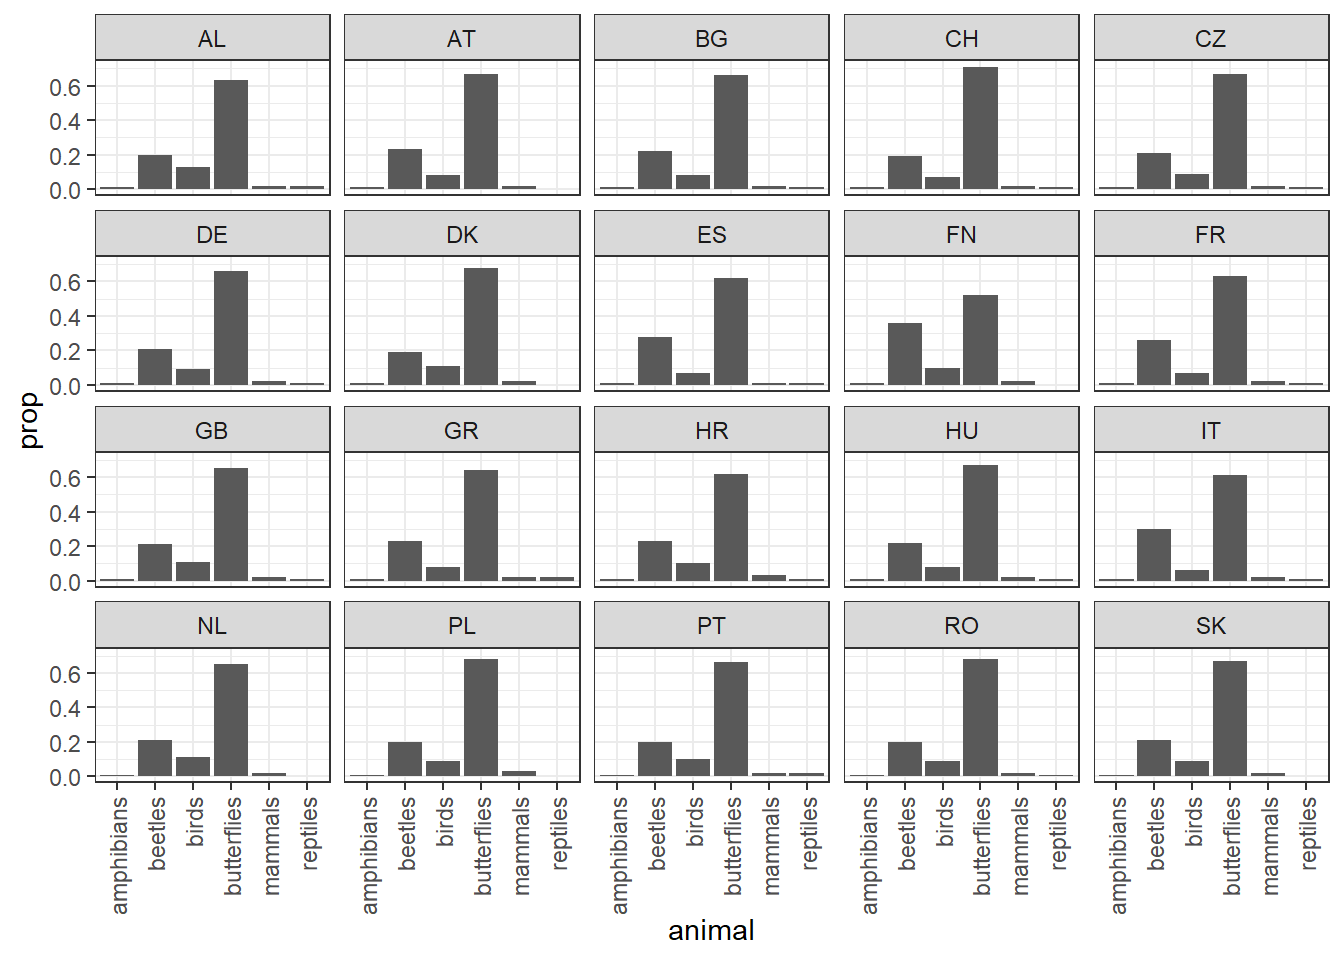
\includegraphics{./cfa_files/figure-pdf/unnamed-chunk-18-1.pdf}

}

\end{figure}

The proportions are pretty stable. Finland seems like the weirdest one,
and it isn't even that weird.

\hypertarget{model-fitting-1}{%
\subsection{Model Fitting}\label{model-fitting-1}}

The hypothesis we want to test here is simply that all of these counts
are confounded by a single unmeasured `biodiversity' variable. This is
straightforward to fit:

\begin{Shaded}
\begin{Highlighting}[]
\NormalTok{h1.definition }\OtherTok{\textless{}{-}} 
\StringTok{\textquotesingle{}diversity =\textasciitilde{} mammals + birds + amphibians + reptiles + beetles + butterflies\textquotesingle{}}

\NormalTok{h1.fit }\OtherTok{\textless{}{-}} \FunctionTok{cfa}\NormalTok{(}
  \AttributeTok{data  =}\NormalTok{ dat\_clean }\SpecialCharTok{\%\textgreater{}\%} \FunctionTok{select}\NormalTok{(}\SpecialCharTok{{-}}\NormalTok{country) }\SpecialCharTok{\%\textgreater{}\%} \FunctionTok{scale}\NormalTok{(),}
  \AttributeTok{model =}\NormalTok{ h1.definition}
\NormalTok{)}

\NormalTok{h1.summary }\OtherTok{\textless{}{-}} \FunctionTok{summary}\NormalTok{(h1.fit)}

\NormalTok{h1.summary}
\end{Highlighting}
\end{Shaded}

\begin{verbatim}
lavaan 0.6-12 ended normally after 23 iterations

  Estimator                                         ML
  Optimization method                           NLMINB
  Number of model parameters                        12

  Number of observations                            20

Model Test User Model:
                                                      
  Test statistic                                20.817
  Degrees of freedom                                 9
  P-value (Chi-square)                           0.013

Parameter Estimates:

  Standard errors                             Standard
  Information                                 Expected
  Information saturated (h1) model          Structured

Latent Variables:
                   Estimate  Std.Err  z-value  P(>|z|)
  diversity =~                                        
    mammals           1.000                           
    birds             0.825    0.277    2.978    0.003
    amphibians        1.115    0.260    4.281    0.000
    reptiles          0.780    0.279    2.793    0.005
    beetles           1.135    0.259    4.380    0.000
    butterflies       1.261    0.254    4.960    0.000

Variances:
                   Estimate  Std.Err  z-value  P(>|z|)
   .mammals           0.387    0.131    2.958    0.003
   .birds             0.566    0.184    3.073    0.002
   .amphibians        0.250    0.092    2.727    0.006
   .reptiles          0.608    0.197    3.089    0.002
   .beetles           0.224    0.085    2.645    0.008
   .butterflies       0.054    0.054    1.010    0.313
    diversity         0.563    0.278    2.025    0.043
\end{verbatim}

Let's have a look at the same 4 goodness-of-fit measures we used in the
previous example. We can bring them all together with a nice utility
function:

\begin{Shaded}
\begin{Highlighting}[]
\DocumentationTok{\#\#\# Define a custom function}
\NormalTok{fit\_measures }\OtherTok{\textless{}{-}} \ControlFlowTok{function}\NormalTok{(fit)\{}
  
\NormalTok{  summary }\OtherTok{\textless{}{-}} \FunctionTok{summary}\NormalTok{(fit, }\AttributeTok{fit.measures =} \ConstantTok{TRUE}\NormalTok{, }\AttributeTok{standardized =} \ConstantTok{TRUE}\NormalTok{)}
  
\NormalTok{  res }\OtherTok{\textless{}{-}} \FunctionTok{list}\NormalTok{(}
    
    \CommentTok{\# Chi{-}Squared}
    \AttributeTok{chi\_squared =} \FunctionTok{tibble}\NormalTok{(}
      \AttributeTok{Test             =} \StringTok{"standard chi{-}squared"}\NormalTok{,}
      \StringTok{\textasciigrave{}}\AttributeTok{DF}\StringTok{\textasciigrave{}}             \OtherTok{=}\NormalTok{ summary}\SpecialCharTok{$}\NormalTok{test}\SpecialCharTok{$}\NormalTok{standard}\SpecialCharTok{$}\NormalTok{df,}
      \StringTok{\textasciigrave{}}\AttributeTok{Test Statistic}\StringTok{\textasciigrave{}} \OtherTok{=} \FunctionTok{round}\NormalTok{(summary}\SpecialCharTok{$}\NormalTok{test}\SpecialCharTok{$}\NormalTok{standard}\SpecialCharTok{$}\NormalTok{stat, }\DecValTok{2}\NormalTok{),}
      \StringTok{\textasciigrave{}}\AttributeTok{p{-}value}\StringTok{\textasciigrave{}}        \OtherTok{=}\NormalTok{ summary}\SpecialCharTok{$}\NormalTok{test}\SpecialCharTok{$}\NormalTok{standard}\SpecialCharTok{$}\NormalTok{pvalue) }\SpecialCharTok{\%\textgreater{}\%} 
      
      \FunctionTok{mutate}\NormalTok{(}\FunctionTok{across}\NormalTok{(}\FunctionTok{everything}\NormalTok{(), as.character)) }\SpecialCharTok{\%\textgreater{}\%} 
      
      \FunctionTok{pivot\_longer}\NormalTok{(}\FunctionTok{everything}\NormalTok{()),}
    
    \CommentTok{\# RMSEA}
    \AttributeTok{rmsea =}\NormalTok{ summary}\SpecialCharTok{$}\NormalTok{fit }\SpecialCharTok{\%\textgreater{}\%} 
      
      \FunctionTok{as\_tibble}\NormalTok{(}\AttributeTok{rownames =} \StringTok{"stat"}\NormalTok{) }\SpecialCharTok{\%\textgreater{}\%} 
      
      \FunctionTok{filter}\NormalTok{(}\FunctionTok{str\_detect}\NormalTok{(stat, }\StringTok{"rmsea"}\NormalTok{)),}
    
    \CommentTok{\# CFI and TLI}
    \AttributeTok{cfi\_tli =}\NormalTok{ summary}\SpecialCharTok{$}\NormalTok{fit }\SpecialCharTok{\%\textgreater{}\%} 
      
      \FunctionTok{as\_tibble}\NormalTok{(}\AttributeTok{rownames =} \StringTok{"stat"}\NormalTok{) }\SpecialCharTok{\%\textgreater{}\%} 
      
      \FunctionTok{filter}\NormalTok{(}\FunctionTok{str\_detect}\NormalTok{(stat, }\StringTok{"cfi|tli"}\NormalTok{)) }
    
\NormalTok{  )}
  
\NormalTok{  res}
  
\NormalTok{\}}

\DocumentationTok{\#\#\# Call the function, then send its outputs to clean tables}
\FunctionTok{fit\_measures}\NormalTok{(h1.fit) }\SpecialCharTok{\%\textgreater{}\%} 
  
  \FunctionTok{map}\NormalTok{(knitr}\SpecialCharTok{::}\NormalTok{kable)}
\end{Highlighting}
\end{Shaded}

\begin{verbatim}
$chi_squared


|name           |value                |
|:--------------|:--------------------|
|Test           |standard chi-squared |
|DF             |9                    |
|Test Statistic |20.82                |
|p-value        |0.0134888288206897   |

$rmsea


|stat           |      value|
|:--------------|----------:|
|rmsea          | 0.25622117|
|rmsea.ci.lower | 0.11034617|
|rmsea.ci.upper | 0.40224444|
|rmsea.pvalue   | 0.01890337|

$cfi_tli


|stat |     value|
|:----|---------:|
|cfi  | 0.8695573|
|tli  | 0.7825955|
\end{verbatim}

The model isn't fitting very well -- Chi-Squared is highly statistically
significant (we fail to reject the null hypothesis that there is
residual variance left to explain), RMSEA is well above its conventional
threshold, and CFI and TLI are both well below their conventional
thresholds.

Here (\textbf{Grace?}) introduces a new method for tweaking our CFA
model to improve goodness of fit. The idea is that we can use fancy math
to ask ``if I took a certain fixed parameter from my model definition
and allowed it to be freely estimated, how much would my model's
chi-squared goodness of fit change?'' People like to take this estimated
change in goodness-of-fit and call it a \textbf{modification index.} As
Brown (2006) puts it:

\begin{quote}
``The modification index reflects an approximation of how much the
overall model \(χ^2\) would decrease if the fixed or constrained
parameter was freely estimated.''
\end{quote}

So to get some ideas on how we might improve our goodness-of-fit, let's
print out the modification indexes for each of the fixed parameters in
the model:

\begin{Shaded}
\begin{Highlighting}[]
\CommentTok{\# Get the estimated change in chi{-}squared for each fixed parameter}
\FunctionTok{modindices}\NormalTok{(h1.fit) }\SpecialCharTok{\%\textgreater{}\%} 
  
  \CommentTok{\# Arrange them in order of modification index}
  \FunctionTok{arrange}\NormalTok{(}\FunctionTok{desc}\NormalTok{(mi)) }\SpecialCharTok{\%\textgreater{}\%} 
  
  \FunctionTok{select}\NormalTok{(lhs, op, rhs, mi) }\SpecialCharTok{\%\textgreater{}\%} 
  
\NormalTok{  knitr}\SpecialCharTok{::}\FunctionTok{kable}\NormalTok{(}\AttributeTok{digits =} \DecValTok{2}\NormalTok{)}
\end{Highlighting}
\end{Shaded}

\begin{longtable}[]{@{}lllr@{}}
\toprule()
lhs & op & rhs & mi \\
\midrule()
\endhead
birds & \textasciitilde\textasciitilde{} & beetles & 4.44 \\
birds & \textasciitilde\textasciitilde{} & amphibians & 3.99 \\
mammals & \textasciitilde\textasciitilde{} & butterflies & 2.84 \\
beetles & \textasciitilde\textasciitilde{} & butterflies & 2.78 \\
mammals & \textasciitilde\textasciitilde{} & amphibians & 2.31 \\
birds & \textasciitilde\textasciitilde{} & reptiles & 2.05 \\
amphibians & \textasciitilde\textasciitilde{} & butterflies & 1.72 \\
birds & \textasciitilde\textasciitilde{} & butterflies & 1.55 \\
mammals & \textasciitilde\textasciitilde{} & reptiles & 1.29 \\
mammals & \textasciitilde\textasciitilde{} & birds & 1.20 \\
amphibians & \textasciitilde\textasciitilde{} & beetles & 0.58 \\
mammals & \textasciitilde\textasciitilde{} & beetles & 0.38 \\
reptiles & \textasciitilde\textasciitilde{} & butterflies & 0.22 \\
reptiles & \textasciitilde\textasciitilde{} & beetles & 0.15 \\
amphibians & \textasciitilde\textasciitilde{} & reptiles & 0.14 \\
\bottomrule()
\end{longtable}

Based on the `ops' symbol ``\textasciitilde\textasciitilde{}'', it seems
like all of the modification indexes correspond to residual correlations
between observed variables. This teaches me something about CFA models!
I guess in the typical CFA model we fix the residual correlations to 0?
This helps me understand why the
\href{https://discourse.mc-stan.org/t/confirmatory-factor-analysis-using-brms/23139}{Bayesian
CFA model as implemented in \textbf{brms}} specifies
\texttt{rescor\ =\ FALSE} . I was confused about this!

Actually, I just realized Gorsuch (1983) already explained this to me!
Think back to where he showed us the definition of the `Common Factor
Model':

\(R_{vv} = PR_{ff}P' + U_{vv}\)

And remember how Gorsuch specified that \(U_{vv}\) is assumed to be a
diagonal matrix, IE the residual correlations is assumed to be
uncorrelated for each variable. This is the whole thing about the
`unique factors', IE the error terms, of the linear models of each
measured variable are gonna be uncorrelated.
\href{https://stats.oarc.ucla.edu/r/seminars/rcfa/}{This recorded
seminar and notes from UCLA} give a nice clear walkthrough of the
notation in a slightly different form from Gorsuch (1983).

From the DAGs perspective of CFA, assuming uncorrelated residuals sort
of makes sense to me: if I want to convince you that my measured
variables are all confounded by the same single unmeasured variable,
then I think fixing the residual errors at 0 is a way of committing my
model to the idea that there aren't \emph{other} unmeasured variables
confounding certain of my measured guys. It is a strong assumption that,
if it holds up, provides better evidence that my variables really truly
are just confounded by a single unmeasured thing.

So I guess I could write out this standard CFA model in a more McElreath
fashion like so:

\$\$ \begin{align*}
\begin{bmatrix} \text{mammals}_i \\ \text{birds}_i \\ \text{amphibians}_i \\ \text{reptiles}_i \\ \text{beetles}_i \\ \end{bmatrix} & \sim
\operatorname{MVNormal} \begin{pmatrix} \begin{bmatrix} \mu_{mammals} \\ \mu_{birds} \\ \mu_{amphibians} \\ \mu_{reptiles} \\ \mu_{beetles} \end{bmatrix}, \mathbf \Sigma\end{pmatrix}\\

\mu_{mammals} = \lambda_{mammals} F_i \\
\mu_{birds} = \lambda_{birds} F_i \\
\mu_{amphibians} = \lambda_{amphibians} F_i \\
\mu_{reptiles} = \lambda_{reptiles} F_i \\
\mu_{beetles} = \lambda_{beetles} F_i \\

\Sigma \begin{pmatrix} 
\sigma_{mammals}&0 &0 &0 &0 \\ 
0 & \sigma_{birds} &0 &0 &0 \\ 
0 & 0 & \sigma_{amphibians} &0 &0 \\ 
0 & 0 & 0 & \sigma_{reptiles} &0 \\ 
0 & 0 & 0 & 0 & \sigma_{beetles} 
\end{pmatrix} \\
\end{align*} \$\$

In human words: the observed counts of each of the 5 animal types are
imagined to be drawn from a shared multivariate normal distribution. The
mean of each dimension of that distribution is a linear function of a
single shared factor, which we're calling `biodiversity'. The variance
of each dimension of that distribution is unique, and there is no
covariance between the dimensions.

But now think back to our modification indexes: a few of them are saying
that if we allow the residual covariances to be freely estimated rather
than fixed at 0, then we can improve model fit by a whole lot.
Specifically, if we allow the residual covariance between birds and
beetles and/or between birds and amphibians to be freely estimated, then
model fit as measured by the chi-squared statistic might be
significantly improved. Here's what the model is gonna look like now:

\$\$ \begin{align*}
\begin{bmatrix} \text{mammals}_i \\ \text{birds}_i \\ \text{amphibians}_i \\ \text{reptiles}_i \\ \text{beetles}_i \\ \end{bmatrix} & \sim
\operatorname{MVNormal} \begin{pmatrix} \begin{bmatrix} \mu_{mammals} \\ \mu_{birds} \\ \mu_{amphibians} \\ \mu_{reptiles} \\ \mu_{beetles} \end{bmatrix}, \mathbf \Sigma\end{pmatrix}\\

\mu_{mammals} = \lambda_{mammals} F_i \\
\mu_{birds} = \lambda_{birds} F_i \\
\mu_{amphibians} = \lambda_{amphibians} F_i \\
\mu_{reptiles} = \lambda_{reptiles} F_i \\
\mu_{beetles} = \lambda_{beetles} F_i \\

\Sigma \begin{pmatrix} 
\sigma_{mammals}&0 &0 &0 &0 \\ 
0 & \sigma_{birds} &\theta_\text{b&a} &0 &\theta_\text{b&b} \\ 
0 &\theta_\text{b&a} & \sigma_{amphibians} &0 &0 \\ 
0 & 0 & 0 & \sigma_{reptiles} &0 \\ 
0 &\theta_\text{b&b} & 0 & 0 & \sigma_{beetles} 
\end{pmatrix} \\
\end{align*} \$\$

See how I've filled in the variance-covariance matrix of the likelihood
to include a few more free parameters?

Actually, Grace proceeds by fitting two more models, one with each of
these two candidate covariance parameters as freely fitting. Then he
uses \texttt{anova()} to do a likelihood-ratio test for them. We can't
test all 3 models at once because models 2 and 3 aren't nested with each
other.

\begin{Shaded}
\begin{Highlighting}[]
\DocumentationTok{\#\#\# Letting the covariance between birds and beetles be freely estimated}
\NormalTok{h2.definition }\OtherTok{\textless{}{-}} 
\StringTok{\textquotesingle{}diversity =\textasciitilde{} mammals + birds + amphibians + }
\StringTok{              reptiles + beetles + butterflies}
\StringTok{ }
\StringTok{ birds \textasciitilde{}\textasciitilde{} beetles\textquotesingle{}}


\NormalTok{h2.fit }\OtherTok{\textless{}{-}} \FunctionTok{cfa}\NormalTok{(}
  \AttributeTok{data  =}\NormalTok{ dat\_clean }\SpecialCharTok{\%\textgreater{}\%} \FunctionTok{select}\NormalTok{(}\SpecialCharTok{{-}}\NormalTok{country) }\SpecialCharTok{\%\textgreater{}\%} \FunctionTok{scale}\NormalTok{(),}
  \AttributeTok{model =}\NormalTok{ h2.definition}
\NormalTok{)}

\NormalTok{h2.summary }\OtherTok{\textless{}{-}} \FunctionTok{summary}\NormalTok{(h2.fit, }\AttributeTok{fit.measures =} \ConstantTok{TRUE}\NormalTok{, }\AttributeTok{standardized =} \ConstantTok{TRUE}\NormalTok{)}

\DocumentationTok{\#\#\# Letting the covariance between birds and amphibians be freely estimated}
\NormalTok{h3.definition }\OtherTok{\textless{}{-}} 
  \StringTok{\textquotesingle{}diversity =\textasciitilde{} mammals + birds + amphibians + }
\StringTok{              reptiles + beetles + butterflies}
\StringTok{ }
\StringTok{ birds \textasciitilde{}\textasciitilde{} amphibians\textquotesingle{}}


\NormalTok{h3.fit }\OtherTok{\textless{}{-}} \FunctionTok{cfa}\NormalTok{(}
 \AttributeTok{data  =}\NormalTok{ dat\_clean }\SpecialCharTok{\%\textgreater{}\%} \FunctionTok{select}\NormalTok{(}\SpecialCharTok{{-}}\NormalTok{country) }\SpecialCharTok{\%\textgreater{}\%} \FunctionTok{scale}\NormalTok{(),}
  \AttributeTok{model =}\NormalTok{ h3.definition}
\NormalTok{)}

\FunctionTok{anova}\NormalTok{(h1.fit, h2.fit)}
\end{Highlighting}
\end{Shaded}

\begin{verbatim}
Chi-Squared Difference Test

       Df    AIC    BIC  Chisq Chisq diff Df diff Pr(>Chisq)  
h2.fit  8 270.81 283.76 16.013                                
h1.fit  9 273.62 285.56 20.817      4.804       1    0.02839 *
---
Signif. codes:  0 '***' 0.001 '**' 0.01 '*' 0.05 '.' 0.1 ' ' 1
\end{verbatim}

\begin{Shaded}
\begin{Highlighting}[]
\FunctionTok{anova}\NormalTok{(h1.fit, h3.fit)}
\end{Highlighting}
\end{Shaded}

\begin{verbatim}
Chi-Squared Difference Test

       Df    AIC    BIC  Chisq Chisq diff Df diff Pr(>Chisq)   
h3.fit  8 267.72 280.67 12.924                                 
h1.fit  9 273.62 285.56 20.817     7.8934       1   0.004961 **
---
Signif. codes:  0 '***' 0.001 '**' 0.01 '*' 0.05 '.' 0.1 ' ' 1
\end{verbatim}

CHOOSE ONE OF THE MODELS, THEN DO CONVERGENT VALIDITY AND RELIABILITY!

\hypertarget{cool-ecology-example-i-should-do-instead}{%
\section{Cool ecology example I should do
instead:}\label{cool-ecology-example-i-should-do-instead}}

\hypertarget{example-3}{%
\section{Example 3:}\label{example-3}}

Do an example from here, or possibly from the linked 3rd lecture that
covers more advanced CFA topics
https://stats.oarc.ucla.edu/r/seminars/rcfa/

Now we'll look at an example from Kline (2011), chapter 13.

Load the data:

\begin{Shaded}
\begin{Highlighting}[]
\NormalTok{dat\_kline }\OtherTok{\textless{}{-}} \FunctionTok{read\_csv}\NormalTok{(}\StringTok{\textquotesingle{}data/kline/kabc{-}amos.csv\textquotesingle{}}\NormalTok{)}
\end{Highlighting}
\end{Shaded}

\begin{verbatim}
Warning: One or more parsing issues, call `problems()` on your data frame for details,
e.g.:
  dat <- vroom(...)
  problems(dat)
\end{verbatim}

\begin{verbatim}
Rows: 11 Columns: 10
-- Column specification --------------------------------------------------------
Delimiter: ","
chr (2): rowtype_, varname_
dbl (8): HM, NR, WO, GC, Tr, SM, MA, PS

i Use `spec()` to retrieve the full column specification for this data.
i Specify the column types or set `show_col_types = FALSE` to quiet this message.
\end{verbatim}

\hypertarget{example-4}{%
\section{Example 4:}\label{example-4}}

Lastly, let's walk through
\href{https://www.lavaan.ugent.be/tutorial/cfa.html}{an example from the
lavaan documentation}

\bookmarksetup{startatroot}

\hypertarget{references}{%
\chapter*{References}\label{references}}
\addcontentsline{toc}{chapter}{References}

\markboth{References}{References}

\hypertarget{refs}{}
\begin{CSLReferences}{1}{0}
\leavevmode\vadjust pre{\hypertarget{ref-Brown2006}{}}%
Brown, Timothy A. 2006. \emph{Confirmatory Factor Analysis for Applied
Research}.

\leavevmode\vadjust pre{\hypertarget{ref-Finch2015}{}}%
Finch, French, W. Holmes. 2015. \emph{Latent Variable Modeling with r}.

\leavevmode\vadjust pre{\hypertarget{ref-gorsuch1983}{}}%
Gorsuch, Richard L. 1983. \emph{Factor Analysis, 2nd Edition}.

\leavevmode\vadjust pre{\hypertarget{ref-Kline2011}{}}%
Kline, Rex B. 2011. \emph{Principles and Practice of Structural Equation
Modeling}.

\end{CSLReferences}



\end{document}
